% ============================================================
% ANEXO A: ESPECIFICACIÓN DE REQUERIMIENTOS DE SOFTWARE (VERSIÓN MEJORADA)
% Traducido y adaptado del ERS completo del primer parcial
% (recursos/informacion-general/main.tex), formato Volere.
% ============================================================

\section{Propósito y Alcance}

\subsection{Definición del Problema}

El almacenamiento de bienes es una necesidad logística recurrente tanto para personas naturales como para empresas, pero la oferta disponible de espacios de almacenamiento está fragmentada y en gran medida subutilizada. Muchos propietarios cuentan con espacios sin uso ---bodegas, garajes, cuartos, contenedores, subsuelos y áticos--- que podrían ofrecerse a terceros, mientras que muchas otras personas y organizaciones tienen dificultad para encontrar alternativas de almacenamiento flexibles, de tamaño adecuado y bien ubicadas. Actualmente, el encuentro entre la oferta y la demanda de espacio de almacenamiento se realiza mayormente por canales informales y sin intermediación, lo que vuelve el proceso lento, opaco y riesgoso para ambas partes.

Esta situación da origen a varios problemas concretos que el presente proyecto de software busca resolver:

\begin{itemize}
    \item \textbf{Falta de confianza e información verificable.} Los posibles arrendatarios no pueden verificar fácilmente las condiciones, dimensiones, ubicación o cumplimiento legal de un espacio de almacenamiento antes de comprometerse a un alquiler, y los propietarios carecen de un mecanismo estructurado de reputación para demostrar confiabilidad.
    \item \textbf{Ausencia de moderación formal y control de cumplimiento.} No existe una autoridad centralizada que valide las publicaciones ---por ejemplo, que el permiso de bomberos obligatorio esté en regla--- antes de que sean expuestas al público.
    \item \textbf{Reserva y contratación ineficientes.} La coordinación de ventanas de disponibilidad, la detección de conflictos de fechas, la formalización del pago y la activación de contratos se realizan manualmente, lo cual es propenso a errores y no escala.
    \item \textbf{Comunicación e incidentes limitados.} Una vez iniciado un alquiler, las partes carecen de un canal dedicado para coordinar el acceso, resolver incidentes o escalar problemas a un moderador, y no existe un flujo estructurado de reporte y resolución.
    \item \textbf{Sin soporte para alquileres organizacionales (a nivel de empresa).} Las empresas que necesitan espacio de almacenamiento para sus colaboradores no pueden gestionar alquileres bajo una identidad colectiva, invitar miembros ni auditar las acciones realizadas en nombre de la organización.
    \item \textbf{Sin acceso móvil.} La gestión de espacios publicados y la exploración de espacios disponibles están limitadas a la experiencia web, lo que restringe el uso en movimiento por parte de propietarios y clientes.
    \item \textbf{Sin integración con sistemas de inventario externos.} Los clientes que ya gestionan su stock en un sistema externo deben volver a ingresar los datos de sus productos manualmente, sin ningún mecanismo para consultar o importar el inventario automáticamente.
\end{itemize}

Para abordar estos problemas, el cliente proporcionó una plataforma web existente, \textbf{Leodega}, como punto de partida del proyecto. Esta plataforma ya ofrece un mercado colaborativo de espacios de almacenamiento ---incluyendo publicación de anuncios, búsqueda, reservas, calificaciones, reportes, moderación, notificaciones y mensajería--- pero debe extenderse con las capacidades organizacionales, móviles, de integración, de cumplimiento y de control especificadas en las historias de usuario, que constituyen la fuente primaria de requerimientos funcionales de este documento.

\subsection{Contexto del Proyecto}

El cliente entregó al equipo una aplicación web \textit{full-stack} ya existente, \textbf{Leodega}, como estado inicial del proyecto. Leodega es un mercado en línea que conecta \textit{landlords} (propietarios de espacios de almacenamiento, en adelante \textbf{Gestores de Almacenamiento}) con \textit{tenants} (arrendatarios, en adelante \textbf{Clientes}), y es supervisado por un \textbf{Administrador del Sistema}. Al momento de la entrega, la plataforma se encontraba en fase de integración y pruebas, y había sido desarrollada bajo la metodología Scrum.

La plataforma heredada está implementada sobre la siguiente base tecnológica, que constituye el cimiento sobre el cual se construyen los requerimientos especificados en este documento:

\begin{itemize}
    \item \textbf{Backend.} Laravel~12 (PHP~8.2+) con autenticación basada en tokens mediante Laravel Sanctum, ORM Eloquent, y base de datos PostgreSQL en producción (SQLite en desarrollo local), containerizado con Docker Compose y desplegable en Railway.
    \item \textbf{Frontend.} React~19 con TypeScript y Vite, React Router DOM con guardas de ruta protegidas y basadas en rol, Tailwind CSS, Axios con interceptor de token \textit{Bearer}, mapas con Leaflet/React-Leaflet, e internacionalización con i18next; desplegable en Vercel.
    \item \textbf{Capacidades existentes.} Autenticación y registro de usuarios, control de acceso basado en roles (administrador, arrendador, arrendatario), publicación y moderación de espacios de almacenamiento, vistas de búsqueda y detalle, reservas con detección de conflictos, calificaciones, reportes, notificaciones dentro de la aplicación, conversaciones y mensajes, un registro de pagos, y paneles según rol.
\end{itemize}

La tarea del equipo es evolucionar esta plataforma heredada para que satisfaga los requerimientos funcionales expresados en las historias de usuario, extendiéndola con cuentas organizacionales, un complemento móvil llamado \textit{Leodeguita}, integración de inventario externo, importación de inventario desde Excel, cumplimiento del permiso de bomberos, un panel de control administrativo, y moderación de cuentas. El sistema opera en un entorno web y requiere conexión a Internet; el complemento Leodeguita extiende las funciones principales a dispositivos móviles.

\subsection{Objetivo General}

Evolucionar la plataforma Leodega hacia un mercado de almacenamiento completo, confiable y accesible desde dispositivos móviles, que conecte a Gestores de Almacenamiento y Clientes ---individualmente o bajo organizaciones--- a través de un sistema moderado y confiable que integre capacidades de reserva, pago, comunicación, reporte de incidentes e integración de inventario, según lo especificado en las historias de usuario.

\subsection{Objetivos Específicos}

Los siguientes objetivos específicos sustentan el objetivo general y corresponden a los grupos de requerimientos funcionales definidos en las historias de usuario:

\begin{enumerate}
    \item \textbf{Gestión de almacenamiento.} Permitir a los Gestores de Almacenamiento registrar, editar y eliminar bodegas ---incluyendo el permiso de bomberos obligatorio--- y ver, cancelar y comunicarse sobre sus reservas. (Referencias: HUG-01 a HUG-08.)
    \item \textbf{Experiencia del cliente.} Permitir a los Clientes buscar y filtrar bodegas, ver su detalle, reservarlas y pagarlas, gestionar sus reservas, comunicarse con los gestores, reportar incidentes, calificar alquileres finalizados, e integrar sus sistemas de inventario externos o importar inventario desde archivos Excel. (Referencias: HUC-01 a HUC-14.)
    \item \textbf{Administración de la plataforma.} Permitir a los Administradores validar permisos de bomberos y moderar publicaciones, bloquear y reactivar cuentas de usuario, monitorear un panel de control con métricas clave, y revisar y resolver reportes. (Referencias: HUA-01 a HUA-04.)
    \item \textbf{Cuentas organizacionales.} Permitir la creación de organizaciones, la invitación y aceptación de clientes como miembros, el cambio entre contextos personal y de organización, las reservas a nivel de empresa, y la administración y auditoría de la actividad organizacional. (Referencias: HUE-01 a HUE-06.)
    \item \textbf{Complemento móvil (Leodeguita).} Proveer acceso móvil para autenticarse con las credenciales de Leodega, seleccionar empresa, publicar bodegas y explorar bodegas disponibles. (Referencias: HUL-01 a HUL-06.)
\end{enumerate}

\subsection{Alcance del Proyecto}

El alcance del sistema está definido por los requerimientos funcionales derivados de las historias de usuario, que se resumen en la Sección~\ref{anexo:ers-resumen} y se detallan en la Sección~\ref{anexo:ers-historias}. La plataforma heredada Leodega provee la base tecnológica y funcional descrita en la sección anterior; la presente especificación rige las capacidades que el sistema entregado debe satisfacer.

\subsubsection*{Alcance funcional por nivel de usuario}

\textbf{Gestor de Almacenamiento (arrendador).} El sistema permite al Gestor: recibir y responder consultas previas a la reserva; recibir notificaciones de confirmación de pago y ver contratos activos; chatear con clientes durante alquileres activos; registrar una bodega con dimensiones, ubicación, fotos, tarifa mensual y permiso de bomberos; ver reservas con filtrado y detalle; cancelar reservas futuras pagadas con una razón obligatoria; eliminar bodegas que no tengan reservas activas o futuras; y editar la información de una bodega. (HUG-01 a HUG-08.)

\textbf{Cliente (arrendatario).} El sistema permite al Cliente: buscar y filtrar bodegas por ubicación, tamaño y precio, con vista de mapa; ver el detalle de una bodega; reservar bodegas disponibles con validación de conflicto de fechas; completar un pago simulado para confirmar una reserva; comunicarse con los gestores antes y durante los alquileres; ver y gestionar reservas activas e históricas; cancelar reservas futuras confirmadas; reportar incidentes; calificar alquileres finalizados; aceptar o rechazar invitaciones a organizaciones; registrar un endpoint de inventario externo y su mapeo de campos; ver el inventario sincronizado; e importar inventario desde un archivo Excel. (HUC-01 a HUC-14.)

\textbf{Administrador.} El sistema permite al Administrador: validar el permiso de bomberos y aprobar o rechazar publicaciones de bodegas; bloquear y reactivar cuentas de usuario con registro de auditoría; monitorear un panel de control con métricas de bodegas, usuarios, transacciones, reservas y reportes sin resolver; y revisar, responder y resolver reportes. (HUA-01 a HUA-04.)

\textbf{Administrador de Organización y miembros de la organización.} El sistema permite a un Administrador de Organización: crear una organización; invitar clientes como miembros; acceder a un panel administrativo empresarial con miembros, reservas e historial; y eliminar reservas empresariales con una razón obligatoria. Permite a los clientes miembros: cambiar entre contexto personal y de organización; reservar en nombre de la organización; y compartir visibilidad de las reservas empresariales, a la vez que se les impide eliminar reservas empresariales. (HUE-01 a HUE-06.)

\textbf{Usuarios de Leodeguita (todos los roles).} El complemento móvil permite a cualquier usuario de Leodega autenticarse con sus credenciales existentes; permite a un cliente seleccionar la empresa operadora; permite a un Gestor de Almacenamiento publicar una bodega para revisión y ver sus bodegas publicadas; y permite a un cliente explorar y ver el detalle de bodegas disponibles. (HUL-01 a HUL-06.)

\subsubsection*{Fuera de alcance}

Los siguientes elementos están explícitamente fuera del alcance de esta especificación:

\begin{itemize}
    \item \textbf{Procesamiento de pagos financieros reales.} El flujo de pago es simulado (HUC-05); no se requiere integración con pasarelas de pago reales ni procesadores bancarios.
    \item \textbf{Integración con ERP y facturación electrónica.} Forman parte de la visión del proyecto pero aún no están implementadas y no están cubiertas por ninguna historia de usuario; quedan excluidas de esta especificación.
    \item \textbf{Una aplicación móvil React Native de propósito general.} Se planifica una aplicación móvil completa para versiones futuras; solo los flujos del complemento Leodeguita especificados en HUL-01 a HUL-06 están en alcance.
    \item \textbf{Funcionalidades de la base heredada no re-especificadas en las historias de usuario} (por ejemplo, favoritos, gestión de tokens de sesión y restablecimiento de contraseña) se conservan de la plataforma heredada tal cual y no se re-especifican como requerimientos funcionales en este documento.
\end{itemize}

\clearpage

\section{Resumen de Requerimientos}
\label{anexo:ers-resumen}

\noindent Este apartado consolida en forma resumida los requerimientos funcionales y no funcionales de la plataforma Leodega. Los requerimientos funcionales se expresan como Historias de Usuario y se detallan en la Sección~\ref{anexo:ers-historias}; los requerimientos no funcionales se detallan en la Sección~\ref{anexo:ers-rnf}. Los resúmenes presentados aquí ofrecen una visión rápida y trazable, y no reemplazan las especificaciones detalladas.

\subsection{Requerimientos Funcionales}

Los requerimientos funcionales del sistema se derivan exclusivamente de las historias de usuario, organizadas por los cinco roles que interactúan con el sistema: \textbf{Gestor de Almacenamiento} (HUG), \textbf{Cliente} (HUC), \textbf{Administrador} (HUA), \textbf{Organización / Empresa} (HUE), y el complemento móvil \textbf{Leodeguita} (HUL). En total, la especificación comprende \textbf{38 requerimientos funcionales}: 8 para el Gestor de Almacenamiento, 14 para el Cliente, 4 para el Administrador, 6 para la Organización y 6 para el complemento móvil Leodeguita.

{\setlength{\tabcolsep}{4pt}
\begin{longtable}{|M{1.8cm}|L{9.5cm}|M{2.3cm}|}
\caption{Resumen de Requerimientos Funcionales} \label{tab:fr-summary} \\
\hline
\rowcolor{cajagris}
\textbf{ID} & \textbf{Nombre del requerimiento} & \textbf{Referencia} \\
\hline
\endfirsthead
\multicolumn{3}{c}{\textit{Tabla~\ref{tab:fr-summary} (continuación)}} \\
\hline
\rowcolor{cajagris}
\textbf{ID} & \textbf{Nombre del requerimiento} & \textbf{Referencia} \\
\hline
\endhead
\hline \multicolumn{3}{r}{\textit{continúa en la siguiente página}} \\
\endfoot
\hline
\endlastfoot

\multicolumn{3}{l}{\textbf{Gestor de Almacenamiento (HUG)}} \\ \hline
HUG-01 & Recepción y respuesta de consultas previas a la reserva & \S\ref{req:HUG-01} \\ \hline
HUG-02 & Notificación de confirmación de pago y activación de contrato & \S\ref{req:HUG-02} \\ \hline
HUG-03 & Chat con clientes durante contrato activo & \S\ref{req:HUG-03} \\ \hline
HUG-04 & Registro de bodega con permiso de bomberos & \S\ref{req:HUG-04} \\ \hline
HUG-05 & Visualización, filtrado y detalle de la lista de reservas & \S\ref{req:HUG-05} \\ \hline
HUG-06 & Cancelación de reservas futuras pagadas & \S\ref{req:HUG-06} \\ \hline
HUG-07 & Eliminación de bodega (sin reservas activas ni futuras) & \S\ref{req:HUG-07} \\ \hline
HUG-08 & Edición de información de bodega & \S\ref{req:HUG-08} \\ \hline

\multicolumn{3}{l}{\textbf{Cliente (HUC)}} \\ \hline
HUC-01 & Búsqueda, filtrado y vista de mapa de bodegas & \S\ref{req:HUC-01} \\ \hline
HUC-02 & Vista de detalle de bodega & \S\ref{req:HUC-02} \\ \hline
HUC-03 & Reserva de bodega con detección de conflicto de fechas & \S\ref{req:HUC-03} \\ \hline
HUC-04 & Mensaje previo a la reserva al gestor & \S\ref{req:HUC-04} \\ \hline
HUC-05 & Confirmación de pago simulado & \S\ref{req:HUC-05} \\ \hline
HUC-06 & Chat de reserva activa & \S\ref{req:HUC-06} \\ \hline
HUC-07 & Gestión y cancelación del historial de reservas & \S\ref{req:HUC-07} \\ \hline
HUC-08 & Reporte y seguimiento de incidentes & \S\ref{req:HUC-08} \\ \hline
HUC-09 & Calificación y reseña de bodega y gestor & \S\ref{req:HUC-09} \\ \hline
HUC-10 & Registro de endpoint de inventario externo & \S\ref{req:HUC-10} \\ \hline
HUC-11 & Mapeo de campos de inventario externo & \S\ref{req:HUC-11} \\ \hline
HUC-12 & Visualización de inventario sincronizado & \S\ref{req:HUC-12} \\ \hline
HUC-13 & Importación de inventario desde Excel & \S\ref{req:HUC-13} \\ \hline
HUC-14 & Aceptación o rechazo de invitación a organización & \S\ref{req:HUC-14} \\ \hline

\multicolumn{3}{l}{\textbf{Administrador (HUA)}} \\ \hline
HUA-01 & Validación del permiso de bomberos & \S\ref{req:HUA-01} \\ \hline
HUA-02 & Panel de control administrativo & \S\ref{req:HUA-02} \\ \hline
HUA-03 & Bloqueo y reactivación de cuentas de usuario & \S\ref{req:HUA-03} \\ \hline
HUA-04 & Revisión y resolución de reportes & \S\ref{req:HUA-04} \\ \hline

\multicolumn{3}{l}{\textbf{Organización / Empresa (HUE)}} \\ \hline
HUE-01 & Invitación de miembros a la organización & \S\ref{req:HUE-01} \\ \hline
HUE-02 & Cambio de contexto personal / organización & \S\ref{req:HUE-02} \\ \hline
HUE-03 & Panel administrativo empresarial & \S\ref{req:HUE-03} \\ \hline
HUE-04 & Creación de organización & \S\ref{req:HUE-04} \\ \hline
HUE-05 & Reserva a nivel empresarial & \S\ref{req:HUE-05} \\ \hline
HUE-06 & Control de eliminación de reserva empresarial & \S\ref{req:HUE-06} \\ \hline

\multicolumn{3}{l}{\textbf{Complemento móvil Leodeguita (HUL)}} \\ \hline
HUL-01 & Inicio de sesión en Leodeguita con credenciales de Leodega & \S\ref{req:HUL-01} \\ \hline
HUL-02 & Selección de empresa en Leodeguita & \S\ref{req:HUL-02} \\ \hline
HUL-03 & Publicación móvil de bodega para revisión & \S\ref{req:HUL-03} \\ \hline
HUL-04 & Lista de bodegas publicadas (móvil) & \S\ref{req:HUL-04} \\ \hline
HUL-05 & Exploración de espacios disponibles (móvil) & \S\ref{req:HUL-05} \\ \hline
HUL-06 & Vista de detalle de bodega (móvil) & \S\ref{req:HUL-06} \\ \hline
\end{longtable}
}

\subsection{Requerimientos No Funcionales}
\label{sec:non-functional-requirements-summary}

Los requerimientos no funcionales del sistema se categorizan según la clasificación de Ian Sommerville, que distingue tres familias de requerimientos de calidad:

\begin{itemize}
    \item \textbf{Requerimientos de producto}, que restringen el comportamiento del propio software (p.\,ej. eficiencia, confiabilidad, usabilidad, seguridad, portabilidad).
    \item \textbf{Requerimientos organizacionales}, que surgen de las políticas, procedimientos y estándares de desarrollo del equipo y la institución (p.\,ej. estándares de implementación y de proceso).
    \item \textbf{Requerimientos externos}, que surgen de factores externos al sistema y a su desarrollo, como obligaciones regulatorias o legislativas.
\end{itemize}

En total se especifican \textbf{11 requerimientos no funcionales}: ocho de producto (RNF-01, RNF-02, RNF-03, RNF-04, RNF-05, RNF-06, RNF-07 y RNF-10), dos organizacionales (RNF-08 y RNF-09), y uno externo (RNF-11). Cada uno se enuncia en términos verificables y se acompaña de criterios de validación cuantitativos, detallados en la Sección~\ref{anexo:ers-rnf}.

{\setlength{\tabcolsep}{4pt}
\begin{longtable}{|M{1.6cm}|L{5.5cm}|M{4.2cm}|M{2.3cm}|}
\caption{Resumen de Requerimientos No Funcionales (clasificación de Sommerville)} \label{tab:nfr-summary} \\
\hline
\rowcolor{cajagris}
\textbf{ID} & \textbf{Nombre del requerimiento} & \textbf{Categoría (Sommerville)} & \textbf{Referencia} \\
\hline
\endfirsthead
\multicolumn{4}{c}{\textit{Tabla~\ref{tab:nfr-summary} (continuación)}} \\
\hline
\rowcolor{cajagris}
\textbf{ID} & \textbf{Nombre del requerimiento} & \textbf{Categoría (Sommerville)} & \textbf{Referencia} \\
\hline
\endhead
\hline \multicolumn{4}{r}{\textit{continúa en la siguiente página}} \\
\endfoot
\hline
\endlastfoot
RNF-01 & Rendimiento (tiempo de respuesta) & Producto -- Eficiencia & \S\ref{req:RNF-01} \\ \hline
RNF-02 & Disponibilidad & Producto -- Confiabilidad & \S\ref{req:RNF-02} \\ \hline
RNF-03 & Seguridad: autenticación & Producto -- Seguridad & \S\ref{req:RNF-03} \\ \hline
RNF-04 & Seguridad: protección de datos & Producto -- Seguridad & \S\ref{req:RNF-04} \\ \hline
RNF-05 & Usabilidad & Producto -- Usabilidad & \S\ref{req:RNF-05} \\ \hline
RNF-06 & Compatibilidad (navegadores y dispositivos) & Producto -- Portabilidad & \S\ref{req:RNF-06} \\ \hline
RNF-07 & Internacionalización & Producto -- Portabilidad & \S\ref{req:RNF-07} \\ \hline
RNF-08 & Mantenibilidad & Organizacional -- Implementación & \S\ref{req:RNF-08} \\ \hline
RNF-09 & Testabilidad & Organizacional -- Implementación & \S\ref{req:RNF-09} \\ \hline
RNF-10 & Escalabilidad & Producto -- Eficiencia & \S\ref{req:RNF-10} \\ \hline
RNF-11 & Auditabilidad & Externo -- Regulatorio & \S\ref{req:RNF-11} \\ \hline
\end{longtable}
}

\clearpage

\section{Historias de Usuario Detalladas}
\label{anexo:ers-historias}

\noindent Se detallan a continuación las 38 historias de usuario, agrupadas por los cinco roles que interactúan con el sistema. Cada historia indica su identificador, prioridad (escala MoSCoW: \textit{Must Have}, \textit{Should Have}, \textit{Could Have}), estimación en puntos de historia y el sprint en que se planificó (consistente con el \textit{Sprint Backlog} de la Sección~A), su enunciado en la forma canónica ``Como \ldots, quiero \ldots, para \ldots'', y sus criterios de aceptación expresados como escenarios numerados de la forma Contexto, Evento y Resultado esperado.

\subsection{Gestor de Almacenamiento (HUG)}

\textbf{HUG-01 -- Recepción y respuesta de consultas previas a la reserva.} \label{req:HUG-01}
\textit{Prioridad:} Could Have \quad \textit{Estimación:} 5 puntos \quad \textit{Sprint:} 4

\textbf{Enunciado.} Como Gestor de Almacenamiento, necesito recibir y responder mensajes de consulta previa de clientes interesados en mis espacios, para brindar información oportuna y generar confianza antes de que el cliente haga una reserva formal.

\textbf{Criterios de aceptación.}
\begin{enumerate}
\item \textbf{Escenario 1: Nueva consulta recibida.} \textit{Contexto:} un cliente envió un mensaje de consulta sobre uno de los espacios del Gestor. \textit{Evento:} el sistema notifica al Gestor sobre el nuevo mensaje. \textit{Resultado esperado:} el sistema muestra la notificación en el panel del Gestor con el nombre del cliente, el espacio consultado y el contenido del mensaje, y el Gestor puede acceder al hilo de conversación desde la notificación.
\item \textbf{Escenario 2: Respuesta exitosa al mensaje del cliente.} \textit{Contexto:} el Gestor accede al hilo de mensajes de un cliente interesado y escribe una respuesta. \textit{Evento:} el Gestor envía el mensaje de respuesta. \textit{Resultado esperado:} el sistema registra y entrega la respuesta al cliente, actualiza el hilo de conversación para ambas partes, y marca la consulta como respondida en el panel del Gestor.
\item \textbf{Escenario 3: Consulta sin responder tras el límite de tiempo.} \textit{Contexto:} el Gestor tiene una o más consultas pendientes que aún no han sido respondidas. \textit{Evento:} el sistema detecta que el plazo transcurrió sin respuesta. \textit{Resultado esperado:} el sistema muestra las consultas sin responder resaltadas como ``pendientes'', ordenadas de más antigua a más reciente, para que el Gestor priorice sus respuestas. El prototipo no define un plazo automático ni una penalización.
\end{enumerate}

\textbf{HUG-02 -- Notificación de confirmación de pago y activación de contrato.} \label{req:HUG-02}
\textit{Prioridad:} Should Have \quad \textit{Estimación:} 3 puntos \quad \textit{Sprint:} 2

\textbf{Enunciado.} Como Gestor de Almacenamiento, necesito recibir una notificación cuando un cliente confirma el pago de una reserva, para saber en tiempo real qué contratos se formalizaron y están listos para iniciar el período de alquiler.

\textbf{Criterios de aceptación.}
\begin{enumerate}
\item \textbf{Escenario 1: Notificación exitosa de pago confirmado.} \textit{Contexto:} un cliente completó el proceso de pago de una reserva sobre uno de los espacios del Gestor. \textit{Evento:} el sistema registra la confirmación de pago del cliente. \textit{Resultado esperado:} el sistema envía una notificación al Gestor con el nombre del cliente, el espacio reservado, el monto pagado y las fechas del contrato, y el contrato pasa a estar activo en el panel del Gestor.
\item \textbf{Escenario 2: Pago no recibido tras el plazo.} \textit{Contexto:} el cliente inició una reserva sobre uno de los espacios del Gestor pero no completó el pago dentro del tiempo de retención. \textit{Evento:} el sistema detecta que el plazo de pago expiró sin confirmación. \textit{Resultado esperado:} el sistema no finaliza la reserva, devuelve el espacio al estado disponible, y notifica al Gestor que el espacio quedó libre nuevamente.
\item \textbf{Escenario 3: Visualización del contrato activo en el panel.} \textit{Contexto:} el Gestor accede al panel de contratos tras recibir la notificación de pago confirmado. \textit{Evento:} el Gestor abre la sección de contratos activos. \textit{Resultado esperado:} el sistema muestra el contrato con todos sus detalles (cliente, espacio, fechas, monto y estado ``Activo''), y el Gestor puede acceder al chat del cliente desde el mismo panel.
\end{enumerate}

\textbf{HUG-03 -- Chat con clientes durante contrato activo.} \label{req:HUG-03}
\textit{Prioridad:} Could Have \quad \textit{Estimación:} 5 puntos \quad \textit{Sprint:} 4

\textbf{Enunciado.} Como Gestor de Almacenamiento, necesito contar con un canal de chat activo con mis clientes durante el período de alquiler vigente, para coordinar accesos, resolver incidentes y mantener comunicación directa sin salir de la plataforma.

\textbf{Criterios de aceptación.}
\begin{enumerate}
\item \textbf{Escenario 1: Envío de mensaje a un cliente con contrato activo.} \textit{Contexto:} el Gestor tiene un contrato activo con un cliente y quiere enviarle un mensaje desde el panel de contratos. \textit{Evento:} el Gestor escribe y envía el mensaje en el chat del contrato. \textit{Resultado esperado:} el sistema registra el mensaje, lo entrega al cliente y actualiza el hilo del chat con la hora de envío, y el cliente recibe una notificación push o en pantalla.
\item \textbf{Escenario 2: Recepción de mensaje del cliente con notificación.} \textit{Contexto:} el cliente envió un mensaje al Gestor a través del chat de un contrato activo. \textit{Evento:} el mensaje del cliente llega al sistema. \textit{Resultado esperado:} el sistema notifica al Gestor con una alerta que indica el nombre del cliente y el contrato asociado, y el Gestor puede responder directamente desde la notificación o desde el panel de contratos.
\item \textbf{Escenario 3: Intento de chatear en un contrato finalizado.} \textit{Contexto:} el Gestor intenta enviar un mensaje a un cliente cuyo contrato de alquiler ya finalizó. \textit{Evento:} el Gestor intenta escribir en el chat de ese contrato. \textit{Resultado esperado:} el sistema deshabilita el campo de texto y muestra: ``Este chat no está disponible porque el período de alquiler ha finalizado.'' El historial permanece visible en modo de solo lectura.
\end{enumerate}

\textbf{HUG-04 -- Registro de bodega con permiso de bomberos.} \label{req:HUG-04}
\textit{Prioridad:} Must Have \quad \textit{Estimación:} 5 puntos \quad \textit{Sprint:} 1

\textbf{Enunciado.} Como Gestor de Almacenamiento, necesito registrar una nueva bodega en la plataforma, incluyendo dimensiones, ubicación, fotos, tarifa mensual y el permiso de bomberos vigente, para ofrecer mi espacio disponible en alquiler.

\textbf{Criterios de aceptación.}
\begin{enumerate}
\item \textbf{Escenario 1: Registro exitoso de bodega con permiso adjunto.} \textit{Contexto:} el Gestor accede al formulario de registro de bodega y cuenta con toda la información requerida del espacio. \textit{Evento:} el Gestor completa todos los campos requeridos, adjunta el permiso de bomberos vigente, y envía el formulario. \textit{Resultado esperado:} el sistema valida los datos, almacena el permiso junto con la bodega, la crea con estado ``pendiente de verificación'', la envía al Administrador para revisión, y muestra un mensaje de éxito.
\item \textbf{Escenario 2: Intento de registro sin adjuntar el permiso.} \textit{Contexto:} el Gestor está completando el formulario de registro de una nueva bodega. \textit{Evento:} el Gestor completa los campos requeridos pero \textit{no} adjunta el permiso de bomberos y envía el formulario. \textit{Resultado esperado:} el sistema bloquea el envío, no crea la bodega, y muestra el mensaje: ``Debe adjuntar el permiso de bomberos vigente para continuar.''
\item \textbf{Escenario 3: Intento de registro con campos requeridos incompletos.} \textit{Contexto:} el Gestor deja uno o más campos requeridos incompletos. \textit{Evento:} el Gestor omite un campo requerido. \textit{Resultado esperado:} el sistema muestra un mensaje de error indicando los campos requeridos y no permite enviar el formulario.
\end{enumerate}

\textbf{HUG-05 -- Visualización, filtrado y detalle de la lista de reservas.} \label{req:HUG-05}
\textit{Prioridad:} Must Have \quad \textit{Estimación:} 3 puntos \quad \textit{Sprint:} 2

\textbf{Enunciado.} Como Gestor de Almacenamiento, necesito ver todas las reservas hechas sobre mis bodegas, con detalle de fechas, cliente y estado de pago, para gestionar el uso de mi espacio y planificar la logística.

\textbf{Criterios de aceptación.}
\begin{enumerate}
\item \textbf{Escenario 1: Visualización de la lista de reservas.} \textit{Contexto:} el Gestor tiene al menos una bodega publicada con reservas registradas. \textit{Evento:} el Gestor accede al módulo de reservas en la página web. \textit{Resultado esperado:} el sistema muestra una tabla con todas las reservas de sus bodegas, incluyendo cliente, bodega, fecha de inicio y fin, estado (pagada o cancelada) y monto.
\item \textbf{Escenario 2: Filtrado y búsqueda de reservas.} \textit{Contexto:} el Gestor está viendo la lista de reservas y quiere acotar los resultados. \textit{Evento:} el Gestor usa filtros por rango de fechas, estado de reserva o nombre de cliente. \textit{Resultado esperado:} el sistema actualiza la lista mostrando solo las reservas que cumplen los criterios seleccionados.
\item \textbf{Escenario 3: Visualización del detalle de una reserva.} \textit{Contexto:} el Gestor está viendo la lista de reservas y quiere ver el detalle de una reserva en particular. \textit{Evento:} el Gestor hace clic sobre una reserva específica. \textit{Resultado esperado:} el sistema abre una vista detallada con la información completa del cliente y el comprobante de pago.
\end{enumerate}

\textbf{HUG-06 -- Cancelación de reservas futuras pagadas.} \label{req:HUG-06}
\textit{Prioridad:} Must Have \quad \textit{Estimación:} 3 puntos \quad \textit{Sprint:} 2

\textbf{Enunciado.} Como Gestor de Almacenamiento, necesito cancelar una reserva previamente pagada, indicando una razón obligatoria, para liberar mi espacio ante imprevistos y mantener transparencia con el cliente.

\textbf{Criterios de aceptación.}
\begin{enumerate}
\item \textbf{Escenario 1: Cancelación exitosa de una reserva futura.} \textit{Contexto:} el Gestor tiene una reserva pagada con fecha de inicio futura sobre una de sus bodegas. \textit{Evento:} el Gestor selecciona una reserva pagada con fecha de inicio futura, ingresa una razón válida, y confirma la cancelación. \textit{Resultado esperado:} el sistema cambia el estado de la reserva a ``cancelada por el gestor'', notifica al cliente por correo electrónico, y libera el espacio para nuevas reservas.
\item \textbf{Escenario 2: Cancelación de una reserva ya iniciada o finalizada.} \textit{Contexto:} el Gestor tiene una reserva pagada cuya fecha de inicio ya pasó o que ya finalizó. \textit{Evento:} el Gestor intenta cancelar esa reserva. \textit{Resultado esperado:} el sistema muestra un mensaje de error indicando que no es posible cancelar reservas en curso o finalizadas.
\item \textbf{Escenario 3: Cancelación sin razón.} \textit{Contexto:} el Gestor selecciona una reserva pagada y futura e intenta cancelarla. \textit{Evento:} el Gestor intenta cancelar sin completar el campo obligatorio de razón. \textit{Resultado esperado:} el sistema no permite la cancelación y resalta el campo de razón como requerido.
\end{enumerate}

\textbf{HUG-07 -- Eliminación de bodega (sin reservas activas ni futuras).} \label{req:HUG-07}
\textit{Prioridad:} Must Have \quad \textit{Estimación:} 3 puntos \quad \textit{Sprint:} 1

\textbf{Enunciado.} Como Gestor de Almacenamiento, necesito eliminar una bodega de la plataforma, siempre que no tenga reservas activas ni futuras, para retirar espacios que ya no ofrezco en alquiler.

\textbf{Criterios de aceptación.}
\begin{enumerate}
\item \textbf{Escenario 1: Eliminación exitosa de una bodega sin reservas.} \textit{Contexto:} el Gestor selecciona una bodega de su propiedad que no tiene reservas activas ni futuras confirmadas. \textit{Evento:} el Gestor selecciona ``Eliminar bodega'' y confirma la acción en el diálogo de confirmación. \textit{Resultado esperado:} el sistema retira la bodega del catálogo público y de los listados del Gestor, la marca como inactiva conservando su historial, y muestra ``La bodega se eliminó correctamente.''
\item \textbf{Escenario 2: Intento de eliminar una bodega con reservas activas o futuras.} \textit{Contexto:} la bodega tiene al menos una reserva en curso o una reserva futura confirmada/pagada. \textit{Evento:} el Gestor intenta eliminarla. \textit{Resultado esperado:} el sistema bloquea la eliminación y muestra ``No puedes eliminar esta bodega porque tiene reservas activas o futuras. Espera a que finalicen o gestiónalas antes de eliminarla'', sin realizar ningún cambio.
\item \textbf{Escenario 3: Eliminación de una bodega con solo reservas finalizadas (históricas).} \textit{Contexto:} la bodega solo tiene reservas ya finalizadas, ninguna activa ni futura. \textit{Evento:} el Gestor confirma la eliminación. \textit{Resultado esperado:} el sistema permite la operación pero conserva el historial de reservas finalizadas para fines de auditoría y reportes; la bodega se marca como inactiva en vez de eliminarse físicamente.
\end{enumerate}

\textbf{HUG-08 -- Edición de información de bodega.} \label{req:HUG-08}
\textit{Prioridad:} Must Have \quad \textit{Estimación:} 5 puntos \quad \textit{Sprint:} 1

\textbf{Enunciado.} Como Gestor de Almacenamiento, necesito editar la información de una bodega que ya publiqué, como dimensiones, descripción, fotos, tarifa mensual y disponibilidad, para mantener actualizada mi oferta sin tener que eliminarla y recrearla.

\textbf{Criterios de aceptación.}
\begin{enumerate}
\item \textbf{Escenario 1: Edición exitosa de los datos de la bodega.} \textit{Contexto:} el Gestor accede a una bodega de su propiedad y modifica uno o más de sus campos editables. \textit{Evento:} el Gestor guarda los cambios con todos los datos válidos. \textit{Resultado esperado:} el sistema valida los datos, actualiza la información de la bodega, refleja los cambios en el catálogo y en los listados del Gestor, y muestra ``Los cambios se guardaron correctamente.''
\item \textbf{Escenario 2: Intento de guardar con campos requeridos faltantes o inválidos.} \textit{Contexto:} el Gestor borra un campo requerido o ingresa un valor inválido (por ejemplo, una tarifa cero o negativa). \textit{Evento:} el Gestor intenta guardar los cambios. \textit{Resultado esperado:} el sistema resalta los campos con errores, muestra un mensaje de validación describiendo qué corregir, y no guarda ningún cambio.
\item \textbf{Escenario 3: Edición de una bodega con reservas activas o futuras.} \textit{Contexto:} el Gestor modifica la tarifa u otros datos de una bodega que ya tiene reservas confirmadas o en curso. \textit{Evento:} el Gestor guarda los cambios. \textit{Resultado esperado:} el sistema aplica los cambios solo a nuevas reservas; las reservas ya confirmadas conservan las condiciones (tarifa y fechas) con las que fueron acordadas, y el sistema informa al Gestor que los cambios no afectan los contratos existentes.
\end{enumerate}

\clearpage
\subsection{Cliente (HUC)}

\textbf{HUC-01 -- Búsqueda, filtrado y vista de mapa de bodegas.} \label{req:HUC-01}
\textit{Prioridad:} Must Have \quad \textit{Estimación:} 5 puntos \quad \textit{Sprint:} 2

\textbf{Enunciado.} Como cliente, necesito buscar y filtrar bodegas disponibles por ubicación, tamaño y precio, para encontrar el espacio de almacenamiento que mejor se ajuste a mis necesidades y presupuesto sin tener que revisar manualmente todas las opciones.

\textbf{Criterios de aceptación.}
\begin{enumerate}
\item \textbf{Escenario 1: Búsqueda con resultados disponibles.} \textit{Contexto:} el cliente ingresa al catálogo de bodegas y aplica filtros de ubicación, tamaño mínimo y rango de precio. \textit{Evento:} el cliente presiona el botón de búsqueda con los filtros seleccionados. \textit{Resultado esperado:} el sistema muestra una lista de bodegas aprobadas que cumplen todos los criterios ingresados, con su nombre, precio mensual, tamaño y distancia estimada, y cada resultado incluye un botón para ver el detalle.
\item \textbf{Escenario 2: Búsqueda sin resultados para los filtros aplicados.} \textit{Contexto:} el cliente aplica filtros cuya combinación no coincide con ninguna bodega disponible en el sistema. \textit{Evento:} el cliente ejecuta la búsqueda con esos criterios. \textit{Resultado esperado:} el sistema muestra ``No encontramos bodegas disponibles con esos criterios. Intenta ampliar tu búsqueda'' sin mostrar resultados vacíos ni errores, y ofrece la opción de limpiar los filtros.
\item \textbf{Escenario 3: Vista de mapa de bodegas.} \textit{Contexto:} el cliente activa la vista de mapa desde el catálogo de bodegas. \textit{Evento:} el sistema carga el mapa interactivo. \textit{Resultado esperado:} el sistema muestra marcadores georreferenciados de las bodegas disponibles en el mapa, y al hacer clic en un marcador se despliega una tarjeta con el nombre, precio mensual y un enlace directo al detalle de esa bodega.
\end{enumerate}

\textbf{HUC-02 -- Vista de detalle de bodega.} \label{req:HUC-02}
\textit{Prioridad:} Must Have \quad \textit{Estimación:} 3 puntos \quad \textit{Sprint:} 2

\textbf{Enunciado.} Como cliente, necesito ver el detalle completo de una bodega antes de decidir reservarla, para evaluar si el espacio cumple mis requisitos de condiciones, capacidad, precio y ubicación antes de comprometerme con una reserva.

\textbf{Criterios de aceptación.}
\begin{enumerate}
\item \textbf{Escenario 1: Carga exitosa del detalle de la bodega.} \textit{Contexto:} el cliente selecciona una bodega desde el catálogo o desde el mapa. \textit{Evento:} el sistema carga la página de detalle de esa bodega. \textit{Resultado esperado:} el sistema muestra el nombre de la bodega, galería de imágenes, descripción, dimensiones (m\textsuperscript{2}), precio mensual, dirección exacta con mapa incrustado, nombre del gestor propietario y disponibilidad, y el botón ``Reservar'' se muestra solo si la bodega tiene estado disponible.
\item \textbf{Escenario 2: Bodega no disponible para reserva.} \textit{Contexto:} el cliente accede al detalle de una bodega cuyo estado actual es ``ocupada'' o ``no disponible''. \textit{Evento:} el sistema carga el detalle de esa bodega. \textit{Resultado esperado:} el sistema muestra toda la información de la bodega pero reemplaza el botón ``Reservar'' por una etiqueta que indica ``Actualmente no disponible'', sin permitir iniciar el flujo de reserva.
\item \textbf{Escenario 3: Intento de acceder a una bodega inexistente.} \textit{Contexto:} el cliente accede a una URL de detalle de bodega con un identificador que no existe o fue eliminado del sistema. \textit{Evento:} el sistema intenta cargar la bodega con ese identificador. \textit{Resultado esperado:} el sistema muestra una página de error con ``Esta bodega no existe o ya no está disponible'', con un enlace que redirige al catálogo principal.
\end{enumerate}

\textbf{HUC-03 -- Reserva de bodega con detección de conflicto de fechas.} \label{req:HUC-03}
\textit{Prioridad:} Must Have \quad \textit{Estimación:} 5 puntos \quad \textit{Sprint:} 2

\textbf{Enunciado.} Como cliente, necesito poder reservar una bodega disponible seleccionando el período de alquiler deseado, para asegurar el espacio de almacenamiento que necesito para las fechas requeridas y recibir confirmación formal del acuerdo.

\textbf{Criterios de aceptación.}
\begin{enumerate}
\item \textbf{Escenario 1: Reserva creada exitosamente.} \textit{Contexto:} el cliente está autenticado, ve una bodega disponible, e ingresa fechas de inicio y fin válidas dentro del calendario de disponibilidad. \textit{Evento:} el cliente confirma la reserva presionando el botón ``Confirmar reserva''. \textit{Resultado esperado:} el sistema crea la reserva en estado ``pendiente de pago'', retiene temporalmente la disponibilidad de la bodega para ese período, y redirige al cliente al flujo de pago, mostrando el resumen de la reserva (bodega, período y monto total) con su número identificador.
\item \textbf{Escenario 2: Intento de reserva con fechas superpuestas.} \textit{Contexto:} el cliente selecciona un rango de fechas que se superpone con una reserva ya confirmada para esa misma bodega. \textit{Evento:} el cliente intenta confirmar la reserva con esas fechas. \textit{Resultado esperado:} el sistema bloquea la operación, muestra ``Las fechas seleccionadas no están disponibles. Elige otro período'', y resalta visualmente los períodos ocupados en el calendario sin crear ningún registro.
\item \textbf{Escenario 3: Intento de reserva sin sesión activa.} \textit{Contexto:} un usuario no autenticado presiona el botón ``Reservar'' en la página de detalle de una bodega. \textit{Evento:} el sistema detecta que no hay sesión activa al intentar iniciar el flujo de reserva. \textit{Resultado esperado:} el sistema redirige al usuario al formulario de inicio de sesión, mostrando ``Debes iniciar sesión para hacer una reserva'', y una vez autenticado lo redirige automáticamente a la misma bodega.
\end{enumerate}

\textbf{HUC-04 -- Mensaje previo a la reserva al gestor.} \label{req:HUC-04}
\textit{Prioridad:} Could Have \quad \textit{Estimación:} 3 puntos \quad \textit{Sprint:} 4

\textbf{Enunciado.} Como cliente, necesito poder enviar un mensaje al gestor de una bodega antes de reservar para aclarar dudas sobre el espacio, para obtener información que no está en la descripción y tomar una decisión de reserva más informada sin comprometerme de antemano.

\textbf{Criterios de aceptación.}
\begin{enumerate}
\item \textbf{Escenario 1: Mensaje enviado exitosamente al gestor.} \textit{Contexto:} el cliente autenticado está viendo el detalle de una bodega y tiene una pregunta específica sobre el espacio. \textit{Evento:} el cliente escribe un mensaje en el formulario de consulta y presiona ``Enviar mensaje''. \textit{Resultado esperado:} el sistema registra el mensaje vinculado a la bodega y al cliente, notifica al gestor mediante una alerta interna, y muestra al cliente la confirmación: ``Tu mensaje fue enviado. El gestor responderá pronto.''
\item \textbf{Escenario 2: El cliente recibe una respuesta del gestor.} \textit{Contexto:} el gestor respondió la consulta previa que el cliente envió sobre su bodega. \textit{Evento:} el cliente accede al módulo ``Mis consultas'' o ingresa a la bodega consultada. \textit{Resultado esperado:} el sistema muestra el hilo de conversación con los mensajes en orden cronológico, identificando a cada participante, y el cliente puede continuar la conversación enviando un mensaje adicional desde el mismo hilo.
\item \textbf{Escenario 3: Intento de consulta sin sesión activa.} \textit{Contexto:} un usuario no autenticado intenta enviar un mensaje de consulta al gestor desde la página de detalle de una bodega. \textit{Evento:} el usuario presiona el botón ``Preguntar al gestor'' sin haber iniciado sesión. \textit{Resultado esperado:} el sistema redirige al formulario de inicio de sesión con ``Debes iniciar sesión para contactar al gestor'', y una vez autenticado redirige automáticamente al detalle de la bodega con el formulario de consulta visible.
\end{enumerate}

\textbf{HUC-05 -- Confirmación de pago simulado.} \label{req:HUC-05}
\textit{Prioridad:} Must Have \quad \textit{Estimación:} 5 puntos \quad \textit{Sprint:} 2

\textbf{Enunciado.} Como cliente, necesito completar un proceso de pago simulado para confirmar y activar oficialmente mi reserva, para formalizar el acuerdo de alquiler y activar la reserva de modo que ambas partes reciban confirmación oficial del contrato.

\textbf{Criterios de aceptación.}
\begin{enumerate}
\item \textbf{Escenario 1: Pago simulado completado exitosamente.} \textit{Contexto:} el cliente tiene una reserva en estado ``pendiente de pago'' y accede al flujo de pago. \textit{Evento:} el cliente revisa el resumen de pago (bodega, período, monto total) y presiona el botón ``Confirmar y pagar''. \textit{Resultado esperado:} el sistema registra el pago simulado, cambia el estado de la reserva a ``confirmada y activa'', notifica al gestor que el pago se completó, y muestra al cliente un comprobante con el número de reserva, bodega, fechas, monto y estado ``PAGADA''.
\item \textbf{Escenario 2: Intento de pago después del plazo.} \textit{Contexto:} el cliente inició una reserva pero abandonó el flujo de pago sin completarlo dentro del tiempo de retención del espacio. \textit{Evento:} el cliente presiona el botón de pago de esa reserva. \textit{Resultado esperado:} el sistema no finaliza la reserva, libera la disponibilidad de la bodega que estaba retenida, y muestra ``No completaste el pago, por lo que la reserva no se finalizó. Puedes iniciar una nueva reserva cuando quieras.''
\item \textbf{Escenario 3: Visualización del comprobante de pago.} \textit{Contexto:} el cliente quiere revisar el comprobante de una reserva que ya pagó y que está activa. \textit{Evento:} el cliente accede al detalle de esa reserva desde su panel ``Mis reservas''. \textit{Resultado esperado:} el sistema muestra el comprobante completo con el número de reserva, nombre de la bodega, nombre del gestor, fechas de inicio y fin, monto total pagado, fecha y hora de pago, y estado ``CONFIRMADA'', y el cliente puede descargar el comprobante en PDF.
\end{enumerate}

\textbf{HUC-06 -- Chat de reserva activa.} \label{req:HUC-06}
\textit{Prioridad:} Could Have \quad \textit{Estimación:} 5 puntos \quad \textit{Sprint:} 4

\textbf{Enunciado.} Como cliente, necesito poder comunicarme con el gestor a través de un chat vinculado a mi reserva activa durante el período de alquiler, para coordinar accesos, reportar problemas menores y resolver situaciones operativas sin necesidad de involucrar al administrador en cada interacción.

\textbf{Criterios de aceptación.}
\begin{enumerate}
\item \textbf{Escenario 1: Envío de mensaje en el chat de una reserva activa.} \textit{Contexto:} el cliente tiene una reserva en estado ``confirmada y activa'' y necesita comunicarse con el gestor. \textit{Evento:} el cliente accede al chat desde el detalle de su reserva activa, escribe un mensaje y presiona ``Enviar''. \textit{Resultado esperado:} el sistema registra el mensaje vinculado a la reserva, lo muestra en el hilo de conversación con la marca de tiempo, y notifica al gestor mediante una alerta interna; el mensaje es visible para ambas partes en orden cronológico.
\item \textbf{Escenario 2: Intento de usar el chat en una reserva no activa.} \textit{Contexto:} el cliente intenta acceder al chat de una reserva que ya finalizó, fue cancelada, o aún está pendiente de confirmación. \textit{Evento:} el cliente navega al detalle de esa reserva e intenta abrir el chat. \textit{Resultado esperado:} el sistema deshabilita el campo de escritura y muestra ``El chat solo está disponible durante el período activo de la reserva'', y el historial de mensajes previos permanece visible en modo de solo lectura.
\item \textbf{Escenario 3: Recepción de un mensaje del gestor en el chat.} \textit{Contexto:} el gestor envió un mensaje al cliente dentro del hilo de chat de una reserva activa. \textit{Evento:} el cliente accede a la plataforma o tiene una sesión activa. \textit{Resultado esperado:} el sistema muestra una notificación de nuevo mensaje en el panel del cliente, y al acceder al chat de la reserva correspondiente el mensaje del gestor aparece en el hilo con su nombre, contenido y marca de tiempo, y se marca automáticamente como leído.
\end{enumerate}

\textbf{HUC-07 -- Gestión y cancelación del historial de reservas.} \label{req:HUC-07}
\textit{Prioridad:} Should Have \quad \textit{Estimación:} 3 puntos \quad \textit{Sprint:} 4

\textbf{Enunciado.} Como cliente, necesito ver y gestionar mis reservas activas e históricas desde mi panel personal, para tener visibilidad y control sobre mis contratos de alquiler vigentes y poder cancelar una reserva cuando ya no la necesite.

\textbf{Criterios de aceptación.}
\begin{enumerate}
\item \textbf{Escenario 1: Visualización del historial de reservas.} \textit{Contexto:} el cliente autenticado accede al módulo ``Mis reservas'' desde su panel personal. \textit{Evento:} el sistema carga la pantalla de reservas del cliente. \textit{Resultado esperado:} el sistema muestra una tabla con todas las reservas del cliente, agrupadas por estado (activa, pendiente, finalizada y cancelada), con el nombre de la bodega, fechas de inicio y fin, precio total y estado actual de cada reserva.
\item \textbf{Escenario 2: Cancelación de una reserva activa.} \textit{Contexto:} el cliente tiene una reserva en estado ``confirmada'' y quiere cancelarla antes de la fecha de inicio. \textit{Evento:} el cliente selecciona la opción ``Cancelar reserva'' y confirma la acción en el diálogo de confirmación. \textit{Resultado esperado:} el sistema cambia el estado de la reserva a ``cancelada'', libera la disponibilidad de la bodega para ese período, notifica al gestor de la cancelación, y refleja el cambio de estado inmediatamente en el panel del cliente.
\item \textbf{Escenario 3: Intento de cancelar una reserva ya iniciada.} \textit{Contexto:} el cliente intenta cancelar una reserva cuya fecha de inicio ya pasó y que está en estado ``en curso''. \textit{Evento:} el cliente presiona el botón de cancelar sobre esa reserva. \textit{Resultado esperado:} el sistema bloquea la cancelación, oculta o deshabilita el botón de cancelar para reservas en curso, y muestra ``Esta reserva ya está en curso y no se puede cancelar desde aquí. Contacta al administrador si tienes un problema.''
\end{enumerate}

\textbf{HUC-08 -- Reporte y seguimiento de incidentes.} \label{req:HUC-08}
\textit{Prioridad:} Could Have \quad \textit{Estimación:} 3 puntos \quad \textit{Sprint:} 4

\textbf{Enunciado.} Como cliente, necesito poder reportar un problema relacionado con una bodega o una reserva activa desde mi panel personal, para notificar al administrador sobre incumplimientos, daños o situaciones anómalas y recibir seguimiento de mi caso sin depender de canales externos.

\textbf{Criterios de aceptación.}
\begin{enumerate}
\item \textbf{Escenario 1: Reporte creado exitosamente.} \textit{Contexto:} el cliente tiene una reserva activa o finalizada y quiere reportar un incidente relacionado con esa bodega. \textit{Evento:} el cliente completa el formulario de reporte (seleccionando el tipo de problema y una descripción obligatoria de al menos 20 caracteres) y presiona ``Enviar reporte''. \textit{Resultado esperado:} el sistema registra el reporte con estado ``pendiente'', vincula el reporte a la reserva y a la bodega correspondiente, notifica al administrador, y muestra al cliente el número de caso generado con ``Tu reporte fue enviado. Te notificaremos sobre su resolución.''
\item \textbf{Escenario 2: Seguimiento del estado de un reporte enviado.} \textit{Contexto:} el cliente envió previamente un reporte y quiere conocer su estado actual. \textit{Evento:} el cliente accede al módulo ``Mis reportes'' desde su panel personal. \textit{Resultado esperado:} el sistema muestra la lista de reportes del cliente con el número de caso, fecha de creación, bodega involucrada, estado actual (pendiente, en revisión o resuelto), y, si el administrador envió un mensaje, un indicador de mensaje nuevo junto al reporte correspondiente.
\item \textbf{Escenario 3: Intento de enviar un reporte sin descripción.} \textit{Contexto:} el cliente intenta enviar un reporte sin completar el campo obligatorio de descripción o con menos de 20 caracteres. \textit{Evento:} el cliente presiona el botón ``Enviar reporte'' con el campo de descripción vacío o insuficiente. \textit{Resultado esperado:} el sistema bloquea el envío, resalta el campo de descripción con un borde rojo, y muestra ``La descripción del problema es obligatoria y debe tener al menos 20 caracteres'', sin crear ningún registro en la base de datos.
\end{enumerate}

\textbf{HUC-09 -- Calificación y reseña de bodega y gestor.} \label{req:HUC-09}
\textit{Prioridad:} Could Have \quad \textit{Estimación:} 3 puntos \quad \textit{Sprint:} 4

\textbf{Enunciado.} Como cliente, necesito poder calificar y dejar una reseña sobre el gestor y la bodega una vez finalizado mi período de alquiler, para compartir mi experiencia con otros usuarios de la plataforma y contribuir a la reputación de los gestores, ayudando a futuros clientes a tomar mejores decisiones.

\textbf{Criterios de aceptación.}
\begin{enumerate}
\item \textbf{Escenario 1: Reseña enviada exitosamente.} \textit{Contexto:} el cliente tiene una reserva en estado ``finalizada'' y aún no ha dejado una reseña para esa bodega. \textit{Evento:} el cliente selecciona una puntuación del 1 al 5, escribe un comentario de al menos 10 caracteres, y presiona ``Enviar reseña''. \textit{Resultado esperado:} el sistema registra la reseña vinculada a la bodega y al gestor, la muestra públicamente en el perfil de la bodega, actualiza la calificación promedio del gestor, y notifica al gestor que recibió una nueva reseña.
\item \textbf{Escenario 2: Intento de reseña sobre una reserva no finalizada.} \textit{Contexto:} el cliente intenta dejar una reseña sobre una bodega cuya reserva aún está activa o no ha alcanzado su fecha de fin. \textit{Evento:} el cliente busca la opción de calificar en esa reserva desde su panel personal. \textit{Resultado esperado:} el sistema no muestra la opción de calificar para reservas que no tengan estado ``finalizada''; si el cliente accede directamente por URL, el sistema muestra ``Solo puedes calificar una bodega una vez finalizado tu período de alquiler.''
\item \textbf{Escenario 3: Intento de dejar una segunda reseña sobre la misma reserva.} \textit{Contexto:} un cliente que ya dejó una reseña sobre una reserva finalizada intenta enviar una segunda reseña para esa misma reserva. \textit{Evento:} el cliente accede al detalle de esa reserva finalizada e intenta calificar de nuevo. \textit{Resultado esperado:} el sistema detecta que ya existe una reseña de ese cliente para esa reserva, oculta el formulario de calificación, y muestra la reseña que ya envió con la opción de verla, pero no de modificarla ni agregar una nueva.
\end{enumerate}

\textbf{HUC-10 -- Registro de endpoint de inventario externo.} \label{req:HUC-10}
\textit{Prioridad:} Should Have \quad \textit{Estimación:} 8 puntos \quad \textit{Sprint:} 5

\textbf{Enunciado.} Como cliente, necesito registrar la URL del endpoint de mi sistema de inventario externo junto con la credencial de acceso que dicho sistema me proporcionó, para que Leodega pueda consultar automáticamente los productos almacenados en mi bodega, sin tener que modificar mi sistema ni cargar los productos manualmente.

\textbf{Criterios de aceptación.}
\begin{enumerate}
\item \textbf{Escenario 1: Configuración de conexión exitosa.} \textit{Contexto:} el cliente tiene al menos una reserva activa y accede a la sección de integraciones de su cuenta. \textit{Evento:} el cliente ingresa la URL del endpoint y la credencial de acceso, y presiona ``Probar y guardar conexión''. \textit{Resultado esperado:} el sistema realiza una consulta de prueba al endpoint; si responde correctamente, guarda la configuración cifrada, muestra ``Conexión verificada y guardada'', y habilita la sincronización de inventario para esa bodega.
\item \textbf{Escenario 2: Endpoint o credencial inválidos.} \textit{Contexto:} la URL no responde, no existe, o el sistema externo rechaza la credencial. \textit{Evento:} el cliente presiona ``Probar y guardar conexión''. \textit{Resultado esperado:} el sistema no guarda la configuración, muestra ``No pudimos conectarnos al endpoint. Verifica la URL y la credencial'', e indica el tipo de error detectado (sin respuesta, no autorizado, o formato inválido).
\item \textbf{Escenario 3: Actualización de una conexión existente.} \textit{Contexto:} el cliente cambia de sistema externo o la empresa modifica la URL o la credencial. \textit{Evento:} el cliente edita los datos de conexión y guarda de nuevo. \textit{Resultado esperado:} el sistema reemplaza la configuración anterior, revalida la conexión, y aplica los nuevos datos a partir de la siguiente consulta de inventario.
\end{enumerate}

\textbf{HUC-11 -- Mapeo de campos de inventario externo.} \label{req:HUC-11}
\textit{Prioridad:} Should Have \quad \textit{Estimación:} 8 puntos \quad \textit{Sprint:} 5

\textbf{Enunciado.} Como cliente, necesito configurar cómo corresponden los campos que devuelve el endpoint de mi sistema externo con los campos de Leodega, para que mis datos de inventario se registren correctamente, sin necesidad de modificar mi sistema ni contactar a un desarrollador.

\textbf{Criterios de aceptación.}
\begin{enumerate}
\item \textbf{Escenario 1: Configuración inicial del mapeo.} \textit{Contexto:} el cliente guardó una conexión válida y accede por primera vez a la configuración de mapeo. \textit{Evento:} el sistema obtiene una muestra de la respuesta del endpoint. \textit{Resultado esperado:} el sistema detecta automáticamente los campos presentes en la respuesta y los muestra en una lista a la izquierda, y a la derecha el cliente asigna a qué campo de Leodega corresponde cada uno (nombre del producto, cantidad, unidad de medida, fecha de vencimiento, etc.).
\item \textbf{Escenario 2: Guardado y validación del mapeo.} \textit{Contexto:} el cliente completó la asignación de campos y presiona guardar. \textit{Evento:} el sistema intenta guardar la configuración. \textit{Resultado esperado:} el sistema valida que los campos requeridos de Leodega (nombre del producto y cantidad) tengan un campo asignado; si falta alguno, indica cuáles son requeridos; si todo está correcto, guarda y confirma con ``Mapeo guardado. Tu inventario se sincronizará en la siguiente consulta.''
\item \textbf{Escenario 3: Modificación del mapeo existente.} \textit{Contexto:} el sistema externo cambia los nombres de sus campos. \textit{Evento:} el cliente actualiza y guarda un nuevo mapeo. \textit{Resultado esperado:} el sistema reemplaza la configuración anterior y aplica el nuevo mapeo a partir de la siguiente consulta de inventario.
\end{enumerate}

\textbf{HUC-12 -- Visualización de inventario sincronizado.} \label{req:HUC-12}
\textit{Prioridad:} Could Have \quad \textit{Estimación:} 5 puntos \quad \textit{Sprint:} 5

\textbf{Enunciado.} Como cliente, necesito ver la lista actualizada de productos almacenados en mi espacio reservado en la plataforma, obtenida directamente de mi sistema externo, para controlar mi inventario sin tener que contactar al gestor de la bodega ni depender de canales externos.

\textbf{Criterios de aceptación.}
\begin{enumerate}
\item \textbf{Escenario 1: Visualización del inventario consultado desde el endpoint.} \textit{Contexto:} el cliente tiene una reserva activa y una conexión válida configurada con su sistema externo. \textit{Evento:} el cliente accede a la vista de inventario de su espacio reservado. \textit{Resultado esperado:} el sistema consulta el endpoint en ese momento, aplica el mapeo configurado, y muestra una tabla con los productos, indicando para cada uno el nombre, cantidad actual, unidad de medida, y la fecha y hora de la consulta.
\item \textbf{Escenario 2: El endpoint no responde o la consulta falla.} \textit{Contexto:} el sistema externo está caído, tarda demasiado en responder, o devuelve un error al momento de la consulta. \textit{Evento:} el cliente accede a la vista de inventario. \textit{Resultado esperado:} el sistema muestra ``No pudimos obtener tu inventario en este momento. Estamos mostrando la última información disponible'' junto con los últimos datos consultados y su fecha; si nunca hubo datos, ofrece reintentar o importar un archivo Excel.
\item \textbf{Escenario 3: Espacio sin conexión configurada aún.} \textit{Contexto:} el cliente tiene una reserva activa pero no ha configurado la conexión con su sistema externo. \textit{Evento:} el cliente accede a la sección de inventario de su espacio. \textit{Resultado esperado:} el sistema muestra ``Aún no has conectado tu sistema de inventario. Configura la conexión o importa un archivo Excel para comenzar'', con acceso directo a ambas opciones.
\end{enumerate}

\textbf{HUC-13 -- Importación de inventario desde Excel.} \label{req:HUC-13}
\textit{Prioridad:} Could Have \quad \textit{Estimación:} 5 puntos \quad \textit{Sprint:} 5

\textbf{Enunciado.} Como cliente, necesito poder subir un archivo Excel con la lista de mis productos directamente a la plataforma, para registrar mi inventario rápidamente cuando mi sistema externo no expone un endpoint, sin tener que ingresar cada producto manualmente ni configurar una integración técnica.

\textbf{Criterios de aceptación.}
\begin{enumerate}
\item \textbf{Escenario 1: Importación exitosa de un archivo válido.} \textit{Contexto:} el cliente tiene una reserva activa y sube un archivo Excel con las columnas requeridas (como mínimo, nombre del producto y cantidad). \textit{Evento:} el cliente confirma la importación. \textit{Resultado esperado:} el sistema procesa el archivo, registra todos los productos en el inventario del espacio correspondiente, y muestra un resumen indicando cuántos productos se importaron correctamente.
\item \textbf{Escenario 2: Archivo con filas incompletas o formato incorrecto.} \textit{Contexto:} el archivo Excel subido tiene filas a las que les falta el nombre del producto o la cantidad. \textit{Evento:} el sistema procesa el archivo. \textit{Resultado esperado:} el sistema importa solo las filas válidas, omite las que tienen errores, y muestra un reporte detallado indicando qué filas fueron ignoradas y por qué, sin cancelar la importación completa.
\item \textbf{Escenario 3: Descarga de una plantilla de ejemplo.} \textit{Contexto:} el cliente no sabe qué estructura debe tener su archivo Excel. \textit{Evento:} el cliente selecciona la opción ``Descargar plantilla'' desde la sección de importación. \textit{Resultado esperado:} el sistema descarga un archivo Excel con las columnas esperadas ya definidas en la primera fila y datos de ejemplo en las filas siguientes, listo para ser reemplazado por el cliente.
\end{enumerate}

\textbf{HUC-14 -- Aceptación o rechazo de invitación a organización.} \label{req:HUC-14}
\textit{Prioridad:} Must Have \quad \textit{Estimación:} 3 puntos \quad \textit{Sprint:} 3

\textbf{Enunciado.} Como cliente, necesito poder aceptar o rechazar una invitación que una organización me envió para unirme como miembro, para decidir si quiero operar bajo el nombre de esa organización dentro de la plataforma.

\textbf{Criterios de aceptación.}
\begin{enumerate}
\item \textbf{Escenario 1: Aceptación exitosa de la invitación.} \textit{Contexto:} el cliente tiene una invitación pendiente de una organización y accede a su panel de notificaciones. \textit{Evento:} el cliente presiona el botón ``Aceptar'' en la invitación recibida. \textit{Resultado esperado:} el sistema vincula al cliente como miembro de la organización, actualiza su perfil, notifica al Administrador de Organización, y habilita el selector de contexto (personal / empresa) en la interfaz del cliente.
\item \textbf{Escenario 2: Rechazo de la invitación.} \textit{Contexto:} el cliente recibe una invitación pero no quiere unirse a esa organización. \textit{Evento:} el cliente presiona el botón ``Rechazar'' en la invitación recibida. \textit{Resultado esperado:} el sistema descarta la invitación, notifica al Administrador de Organización que fue rechazada, y no realiza ningún cambio en el perfil ni en los permisos del cliente.
\item \textbf{Escenario 3: Invitación expirada.} \textit{Contexto:} el cliente intenta responder a una invitación que ya superó el período de validez del sistema. \textit{Evento:} el cliente presiona ``Aceptar'' o ``Rechazar'' sobre una invitación expirada. \textit{Resultado esperado:} el sistema muestra ``Esta invitación ya no está disponible. Pide al administrador de la organización que te envíe una nueva'' y archiva automáticamente la invitación.
\end{enumerate}

\clearpage
\subsection{Administrador (HUA)}

\textbf{HUA-01 -- Validación del permiso de bomberos.} \label{req:HUA-01}
\textit{Prioridad:} Could Have \quad \textit{Estimación:} 5 puntos \quad \textit{Sprint:} 1

\textbf{Enunciado.} Como administrador, necesito revisar y validar el documento vigente de permiso de bomberos que el gestor de la bodega subió al sistema, para asegurar el cumplimiento del requisito legal obligatorio antes de habilitar cualquier espacio de almacenamiento en la plataforma.

\textbf{Criterios de aceptación.}
\begin{enumerate}
\item \textbf{Escenario 1: Aprobación con documento válido.} \textit{Contexto:} un gestor envió una solicitud de publicación de bodega y adjuntó un documento de permiso de bomberos válido. \textit{Evento:} el administrador revisa el documento, verifica su validez, y selecciona la opción de aprobar. \textit{Resultado esperado:} el sistema cambia el estado de la bodega a ``aprobada'', la hace visible en el catálogo público, y envía una notificación al gestor informándole que su espacio fue habilitado.
\item \textbf{Escenario 2: Rechazo por documento vencido o inválido.} \textit{Contexto:} el administrador revisa el permiso adjunto y determina que está vencido o no corresponde a la propiedad declarada. \textit{Evento:} el administrador selecciona la opción de rechazar e ingresa una razón obligatoria. \textit{Resultado esperado:} el sistema mantiene la bodega en estado ``rechazada'', impide que sea visible en el catálogo, y envía una notificación al gestor con la razón del rechazo, indicando que debe subir un documento válido para reiniciar el proceso.
\item \textbf{Escenario 3: Solicitud enviada sin documento adjunto.} \textit{Contexto:} un gestor intenta enviar su solicitud de publicación de bodega sin haber subido el permiso de bomberos. \textit{Evento:} el gestor presiona el botón final de envío en el flujo de registro de bodega. \textit{Resultado esperado:} el sistema bloquea el envío, no crea el registro de la bodega, y muestra ``Debe adjuntar el permiso de bomberos vigente para continuar.''
\end{enumerate}

\textbf{HUA-02 -- Panel de control administrativo.} \label{req:HUA-02}
\textit{Prioridad:} Could Have \quad \textit{Estimación:} 8 puntos \quad \textit{Sprint:} 5

\textbf{Enunciado.} Como administrador, necesito ver un panel de control con métricas clave sobre el estado de la plataforma, para tomar decisiones informadas sobre la operación del negocio y monitorear la rentabilidad mensual generada.

\textbf{Criterios de aceptación.}
\begin{enumerate}
\item \textbf{Escenario 1: Carga del panel con métricas generales.} \textit{Contexto:} el administrador ingresa al módulo de panel de control desde el menú principal. \textit{Evento:} el administrador accede al panel y el sistema carga la pantalla. \textit{Resultado esperado:} el sistema muestra tarjetas resumen con el total de bodegas registradas (desglosadas por estado: aprobadas, pendientes y rechazadas), el total de usuarios activos desglosado por rol (gestor y cliente), el monto total transaccionado, y el total de reservas en curso en ese momento.
\item \textbf{Escenario 2: Consulta del flujo de reservas por período.} \textit{Contexto:} el administrador selecciona un mes y año específicos en el filtro de tiempo del panel. \textit{Evento:} el administrador aplica el filtro. \textit{Resultado esperado:} el sistema actualiza las métricas mostrando el número de reservas confirmadas en ese período, el monto total transaccionado, y un gráfico de barras o líneas comparando ese período con el mes anterior.
\item \textbf{Escenario 3: Indicador de reportes sin resolver.} \textit{Contexto:} existen reportes con estado ``pendiente'' registrados en el sistema. \textit{Evento:} el administrador accede al panel de control. \textit{Resultado esperado:} el sistema muestra un indicador numérico de reportes sin resolver clasificados por prioridad (alta, media y baja), con un enlace directo al módulo de gestión de reportes.
\end{enumerate}

\textbf{HUA-03 -- Bloqueo y reactivación de cuentas de usuario.} \label{req:HUA-03}
\textit{Prioridad:} Must Have \quad \textit{Estimación:} 5 puntos \quad \textit{Sprint:} 1

\textbf{Enunciado.} Como administrador, necesito poder bloquear o reactivar cuentas de usuario registradas en la plataforma desde un panel de gestión dedicado, para actuar como moderador ante incumplimientos de las políticas de uso y proteger la integridad de la comunidad.

\textbf{Criterios de aceptación.}
\begin{enumerate}
\item \textbf{Escenario 1: Bloqueo de una cuenta activa.} \textit{Contexto:} el administrador identificó un usuario que violó las políticas de la plataforma y selecciona su perfil en el panel de gestión de usuarios. \textit{Evento:} el administrador confirma la acción de bloqueo e ingresa la razón obligatoria del bloqueo. \textit{Resultado esperado:} el sistema cambia el estado del usuario a ``bloqueado'', invalida inmediatamente todos sus tokens de acceso activos, registra la acción en el log de auditoría con la razón ingresada, y notifica al usuario que su cuenta fue suspendida.
\item \textbf{Escenario 2: Intento de inicio de sesión de un usuario bloqueado.} \textit{Contexto:} un usuario con estado ``bloqueado'' intenta autenticarse en la plataforma con credenciales correctas. \textit{Evento:} el usuario ingresa su correo y contraseña y presiona ``Iniciar sesión''. \textit{Resultado esperado:} el sistema rechaza el acceso y muestra ``Tu cuenta ha sido suspendida. Contacta a soporte para más información'', sin revelar si las credenciales son válidas o incorrectas.
\item \textbf{Escenario 3: Reactivación de una cuenta bloqueada.} \textit{Contexto:} el administrador decide reactivar la cuenta de un usuario que fue bloqueado previamente y cuya situación ya se resolvió. \textit{Evento:} el administrador selecciona la opción de reactivar cuenta desde el panel de gestión. \textit{Resultado esperado:} el sistema cambia el estado del usuario a ``activo'', registra la reactivación en el log de auditoría, y permite al usuario iniciar sesión normalmente en su siguiente intento.
\end{enumerate}

\textbf{HUA-04 -- Revisión y resolución de reportes.} \label{req:HUA-04}
\textit{Prioridad:} Could Have \quad \textit{Estimación:} 3 puntos \quad \textit{Sprint:} 4

\textbf{Enunciado.} Como administrador, necesito revisar y dar seguimiento a los reportes que los clientes envían sobre bodegas o reservas, pudiendo responderlos y cambiar su estado, para gestionar incidentes, mantener la calidad del servicio y cerrar el ciclo de cada reporte.

\textbf{Criterios de aceptación.}
\begin{enumerate}
\item \textbf{Escenario 1: Revisión de un reporte pendiente.} \textit{Contexto:} existe al menos un reporte con estado ``pendiente'' enviado por un cliente. \textit{Evento:} el administrador accede al módulo de gestión de reportes y abre uno. \textit{Resultado esperado:} el sistema muestra el detalle del reporte (tipo, descripción, bodega y reserva vinculadas, cliente y fecha) y permite cambiar su estado a ``en revisión''.
\item \textbf{Escenario 2: Respuesta y resolución del reporte.} \textit{Contexto:} el administrador revisó un reporte y tiene una respuesta o resolución. \textit{Evento:} el administrador escribe un mensaje al cliente y marca el reporte como ``resuelto''. \textit{Resultado esperado:} el sistema cambia el estado a ``resuelto'', registra la respuesta, notifica al cliente con un indicador de mensaje nuevo, y descuenta el reporte del contador de pendientes del panel.
\item \textbf{Escenario 3: Intento de resolver sin respuesta.} \textit{Contexto:} el administrador intenta marcar un reporte como ``resuelto'' sin haber ingresado una respuesta para el cliente. \textit{Evento:} el administrador confirma la resolución con el campo de respuesta vacío. \textit{Resultado esperado:} el sistema bloquea la acción y solicita ingresar una respuesta antes de cerrar el reporte.
\end{enumerate}

\clearpage
\subsection{Organización / Empresa (HUE)}

\textbf{HUE-01 -- Invitación de miembros a la organización.} \label{req:HUE-01}
\textit{Prioridad:} Must Have \quad \textit{Estimación:} 5 puntos \quad \textit{Sprint:} 3

\textbf{Enunciado.} Como Administrador de Organización, necesito poder invitar a usuarios registrados como clientes a unirse a mi organización como miembros, para que mis colaboradores puedan operar bajo el nombre de la empresa en la plataforma.

\textbf{Criterios de aceptación.}
\begin{enumerate}
\item \textbf{Escenario 1: Invitación enviada exitosamente.} \textit{Contexto:} el Administrador busca a un usuario por correo electrónico y el usuario existe con rol de cliente. \textit{Evento:} el administrador selecciona al usuario y confirma el envío de la invitación. \textit{Resultado esperado:} el sistema registra la invitación con estado ``pendiente'' y notifica al cliente mediante una alerta en su panel y un correo con el nombre de la organización y botones para aceptar o rechazar.
\item \textbf{Escenario 2: Intento de invitar a un gestor de bodegas.} \textit{Contexto:} el Administrador intenta buscar e invitar a un usuario con rol de Gestor de Almacenamiento. \textit{Evento:} el administrador ingresa el correo de un gestor en la búsqueda de invitación. \textit{Resultado esperado:} el sistema bloquea la acción y muestra ``Solo puedes invitar a usuarios con rol de cliente. Los gestores de bodegas no pueden unirse a organizaciones.''
\item \textbf{Escenario 3: Intento de invitar a un usuario que ya es miembro.} \textit{Contexto:} el cliente que se está invitando ya es miembro activo de la organización. \textit{Evento:} el administrador selecciona a ese usuario y confirma la invitación. \textit{Resultado esperado:} el sistema muestra ``Este usuario ya es miembro de tu organización'' y no genera un registro de invitación duplicado.
\end{enumerate}

\textbf{HUE-02 -- Cambio de contexto personal / organización.} \label{req:HUE-02}
\textit{Prioridad:} Must Have \quad \textit{Estimación:} 5 puntos \quad \textit{Sprint:} 3

\textbf{Enunciado.} Como Cliente (perteneciente a una organización), necesito poder cambiar entre mi contexto personal y el de cada organización desde un selector visible en la interfaz web, para operar bajo el nombre correcto según la situación, sin necesidad de cerrar sesión ni crear cuentas separadas.

\textbf{Criterios de aceptación.}
\begin{enumerate}
\item \textbf{Escenario 1: Cambio de contexto personal a organización.} \textit{Contexto:} el cliente tiene una sesión activa en contexto personal y pertenece al menos a una organización. \textit{Evento:} el cliente hace clic en el selector de contexto (indicador circular en la esquina superior derecha) y elige el nombre de una organización. \textit{Resultado esperado:} el sistema cambia el contexto activo, actualiza el indicador visual con el nombre/logo de la organización, y recarga el panel mostrando solo las bodegas, reservas e inventario de esa organización.
\item \textbf{Escenario 2: Cambio de contexto de organización a personal.} \textit{Contexto:} el cliente está operando bajo el contexto de una organización. \textit{Evento:} el cliente selecciona ``Modo personal'' desde el selector de contexto. \textit{Resultado esperado:} el sistema restaura el contexto individual, oculta el indicador de organización, y muestra el panel personal con sus propias reservas y actividad.
\item \textbf{Escenario 3: Inicio de sesión con una única organización vinculada.} \textit{Contexto:} el cliente pertenece exactamente a una organización. \textit{Evento:} el cliente inicia sesión en la plataforma. \textit{Resultado esperado:} el sistema muestra el selector de contexto preseleccionado en ``Modo personal'', con la opción de cambiar a la organización visible en la esquina superior derecha, y no redirige automáticamente al contexto empresarial.
\end{enumerate}

\textbf{HUE-03 -- Panel administrativo empresarial.} \label{req:HUE-03}
\textit{Prioridad:} Should Have \quad \textit{Estimación:} 5 puntos \quad \textit{Sprint:} 3

\textbf{Enunciado.} Como Administrador de Organización, necesito acceder a un panel administrativo empresarial donde pueda ver los miembros, reservas activas e historial de la organización, para tener visibilidad y control completos sobre las operaciones realizadas a nombre de mi empresa.

\textbf{Criterios de aceptación.}
\begin{enumerate}
\item \textbf{Escenario 1: Carga del panel administrativo empresarial.} \textit{Contexto:} el Administrador de Organización inicia sesión o cambia al contexto empresarial. \textit{Evento:} el administrador accede al panel de administración de la organización. \textit{Resultado esperado:} el sistema muestra un resumen con el número de miembros activos, reservas vigentes, historial de reservas, e invitaciones pendientes de respuesta.
\item \textbf{Escenario 2: Gestión de miembros: eliminar un miembro.} \textit{Contexto:} el Administrador quiere remover a un cliente de la organización. \textit{Evento:} el administrador selecciona a un miembro de la lista y confirma su remoción. \textit{Resultado esperado:} el sistema desvincula al cliente de la organización, elimina su acceso al panel empresarial, notifica al cliente, y conserva el historial de reservas que hizo mientras fue miembro.
\item \textbf{Escenario 3: Visualización del historial de acciones de la organización.} \textit{Contexto:} el Administrador quiere auditar las acciones realizadas a nombre de la empresa. \textit{Evento:} el administrador accede a la sección de historial del panel empresarial. \textit{Resultado esperado:} el sistema muestra un registro cronológico de reservas creadas/canceladas y miembros agregados/eliminados, indicando en cada entrada el nombre del miembro que realizó la acción y la fecha.
\end{enumerate}

\textbf{HUE-04 -- Creación de organización.} \label{req:HUE-04}
\textit{Prioridad:} Must Have \quad \textit{Estimación:} 5 puntos \quad \textit{Sprint:} 3

\textbf{Enunciado.} Como Administrador de Organización, necesito poder crear una organización desde mi cuenta de cliente, ingresando los datos de la empresa (razón social, RUC y correo de la organización), para gestionar alquileres de bodega a nombre de mi organización, sin tener que crear una cuenta separada.

\textbf{Criterios de aceptación.}
\begin{enumerate}
\item \textbf{Escenario 1: Registro exitoso de la organización.} \textit{Contexto:} un cliente con sesión activa completa los datos requeridos de la organización (razón social, RUC de 13 dígitos y correo de la organización). \textit{Evento:} el usuario presiona el botón ``Crear organización''. \textit{Resultado esperado:} el sistema valida el RUC (13 dígitos y único en el sistema), crea la organización vinculada a la cuenta del cliente y lo designa como Administrador de Organización (sin dejar de ser cliente), la activa automáticamente, genera el panel administrativo empresarial, y habilita el selector de contexto personal/empresa.
\item \textbf{Escenario 2: Intento de registro con un RUC ya existente.} \textit{Contexto:} el RUC ingresado ya está registrado en el sistema por otra organización. \textit{Evento:} el usuario intenta enviar el formulario con ese RUC. \textit{Resultado esperado:} el sistema bloquea el envío, resalta el campo de RUC, y muestra ``Ya existe una organización registrada con este RUC. Si crees que esto es un error, contacta a soporte.''
\item \textbf{Escenario 3: Intento de registro con campos requeridos faltantes.} \textit{Contexto:} el usuario omite uno o más campos requeridos del formulario. \textit{Evento:} el usuario intenta enviar el formulario incompleto. \textit{Resultado esperado:} el sistema resalta en rojo cada campo requerido vacío y muestra mensajes de validación individuales, y no se crea ningún registro hasta que se completen todos los campos requeridos.
\end{enumerate}

\textbf{HUE-05 -- Reserva a nivel empresarial.} \label{req:HUE-05}
\textit{Prioridad:} Must Have \quad \textit{Estimación:} 5 puntos \quad \textit{Sprint:} 3

\textbf{Enunciado.} Como Cliente (perteneciente a una organización), necesito poder reservar una bodega disponible a nombre de la organización a la que pertenezco, para asegurar espacio de almacenamiento para la empresa y que todos los miembros puedan ver y gestionar esa reserva.

\textbf{Criterios de aceptación.}
\begin{enumerate}
\item \textbf{Escenario 1: Reserva empresarial creada exitosamente.} \textit{Contexto:} el cliente tiene activo el contexto de una organización, ve una bodega disponible, e ingresa fechas válidas. \textit{Evento:} el cliente confirma la reserva presionando ``Confirmar reserva''. \textit{Resultado esperado:} el sistema crea la reserva vinculada a la organización (no al cliente individual), notifica al gestor de la bodega, y actualiza el panel de todos los miembros activos de esa organización para que vean la nueva reserva.
\item \textbf{Escenario 2: Visualización compartida de la reserva por otro miembro.} \textit{Contexto:} un segundo cliente miembro accede al panel empresarial después de que se hizo una reserva. \textit{Evento:} el segundo miembro navega a la sección de reservas en el contexto de la organización. \textit{Resultado esperado:} el sistema muestra la reserva con todos sus detalles, indicando el nombre del miembro que la realizó, y ambos pueden acceder al chat de la reserva.
\item \textbf{Escenario 3: Intento de reserva sin contexto empresarial activo.} \textit{Contexto:} el cliente miembro está operando en su contexto personal e intenta reservar una bodega. \textit{Evento:} el cliente confirma la reserva en contexto personal. \textit{Resultado esperado:} el sistema procesa la reserva como una reserva personal del cliente, no como una empresarial, y la reserva no aparece en el panel de la organización.
\end{enumerate}

\textbf{HUE-06 -- Control de eliminación de reserva empresarial.} \label{req:HUE-06}
\textit{Prioridad:} Must Have \quad \textit{Estimación:} 3 puntos \quad \textit{Sprint:} 3

\textbf{Enunciado.} Como Cliente (perteneciente a una organización), necesito que el sistema me impida eliminar bodegas reservadas bajo la organización, ya que esa acción está reservada al Administrador de Organización, para proteger los contratos empresariales de eliminaciones accidentales o no autorizadas por parte de miembros sin permisos suficientes.

\textbf{Criterios de aceptación.}
\begin{enumerate}
\item \textbf{Escenario 1: Botón de eliminar no disponible para un miembro.} \textit{Contexto:} un cliente miembro accede al detalle de una reserva empresarial activa. \textit{Evento:} el miembro visualiza las opciones disponibles en esa vista de detalle de reserva. \textit{Resultado esperado:} el sistema no muestra el botón ``Eliminar reserva'' para el cliente miembro, y solo se muestran las opciones de ver detalles y acceder al chat de la reserva.
\item \textbf{Escenario 2: El administrador de organización puede eliminar una reserva.} \textit{Contexto:} el Administrador de Organización accede al detalle de una reserva empresarial activa. \textit{Evento:} el administrador selecciona ``Eliminar reserva'', ingresa una razón obligatoria, y confirma la acción. \textit{Resultado esperado:} el sistema cancela la reserva, libera la bodega, notifica al gestor y a todos los miembros de la organización sobre la cancelación, y registra la razón en el historial de la empresa.
\item \textbf{Escenario 3: Intento de eliminación por un miembro mediante URL directa.} \textit{Contexto:} un cliente miembro intenta acceder a la acción de eliminar manipulando la URL. \textit{Evento:} el sistema recibe la solicitud de eliminación con el token del cliente miembro. \textit{Resultado esperado:} el sistema rechaza la operación con un error 403, no realiza cambios en la base de datos, y registra el intento fallido en el log de auditoría.
\end{enumerate}

\clearpage
\subsection{Leodeguita, complemento móvil (HUL)}

\textbf{HUL-01 -- Inicio de sesión en Leodeguita con credenciales de Leodega.} \label{req:HUL-01}
\textit{Prioridad:} Must Have \quad \textit{Estimación:} 3 puntos \quad \textit{Sprint:} 1

\textbf{Enunciado.} Como usuario (administrador, gestor de bodega o cliente), necesito iniciar sesión en Leodeguita con mis credenciales de Leodega, para acceder a mis datos y funcionalidades sin necesidad de crear una cuenta separada.

\textbf{Criterios de aceptación.}
\begin{enumerate}
\item \textbf{Escenario 1: Inicio de sesión exitoso.} \textit{Contexto:} el usuario tiene una cuenta activa en Leodega. \textit{Evento:} ingresa su correo y contraseña correctamente y presiona ``Iniciar sesión''. \textit{Resultado esperado:} el sistema autentica al usuario y lo redirige a la pantalla principal correspondiente a su rol.
\item \textbf{Escenario 2: Credenciales incorrectas.} \textit{Contexto:} el usuario ingresa un correo o contraseña que no coincide con ninguna cuenta registrada. \textit{Evento:} presiona ``Iniciar sesión''. \textit{Resultado esperado:} el sistema muestra un mensaje de error indicando que las credenciales son incorrectas y no permite el acceso.
\item \textbf{Escenario 3: Campos requeridos vacíos.} \textit{Contexto:} el usuario deja en blanco el campo de correo o de contraseña. \textit{Evento:} presiona ``Iniciar sesión''. \textit{Resultado esperado:} el sistema resalta los campos vacíos, muestra un mensaje indicando que son requeridos, y no intenta autenticar.
\end{enumerate}

\textbf{HUL-02 -- Selección de empresa en Leodeguita.} \label{req:HUL-02}
\textit{Prioridad:} Must Have \quad \textit{Estimación:} 3 puntos \quad \textit{Sprint:} 3

\textbf{Enunciado.} Como cliente, necesito seleccionar la empresa bajo la cual quiero operar dentro de Leodeguita, para ver solo las bodegas y elementos correspondientes a esa empresa.

\textbf{Criterios de aceptación.}
\begin{enumerate}
\item \textbf{Escenario 1: Cliente con múltiples empresas.} \textit{Contexto:} el cliente está asociado a más de una empresa en el sistema. \textit{Evento:} accede al selector de empresa y elige una distinta a la activa. \textit{Resultado esperado:} el sistema actualiza toda la vista para mostrar solo las bodegas y elementos correspondientes a la empresa seleccionada.
\item \textbf{Escenario 2: Cliente con una sola empresa.} \textit{Contexto:} el cliente está asociado a una única empresa. \textit{Evento:} inicia sesión en Leodeguita. \textit{Resultado esperado:} el sistema establece automáticamente esa empresa como activa y no muestra el selector de empresa.
\item \textbf{Escenario 3: Cliente sin empresas asociadas.} \textit{Contexto:} el cliente no está asociado a ninguna empresa en el sistema. \textit{Evento:} inicia sesión en Leodeguita. \textit{Resultado esperado:} el sistema redirige al usuario a la vista correspondiente al rol de cliente.
\end{enumerate}

\textbf{HUL-03 -- Publicación móvil de bodega para revisión.} \label{req:HUL-03}
\textit{Prioridad:} Must Have \quad \textit{Estimación:} 5 puntos \quad \textit{Sprint:} 1

\textbf{Enunciado.} Como gestor de bodega, necesito registrar un espacio de bodega disponible para alquiler con la menor cantidad de pasos posible, para ofrecerlo a los clientes rápidamente desde mi dispositivo móvil.

\textbf{Criterios de aceptación.}
\begin{enumerate}
\item \textbf{Escenario 1: Envío exitoso para revisión.} \textit{Contexto:} el gestor completó todos los campos requeridos del formulario. \textit{Evento:} presiona ``Publicar espacio''. \textit{Resultado esperado:} el sistema registra la bodega en el backend, la crea con estado ``pendiente de verificación'', y la envía al Administrador para revisión; la bodega \textit{no} es visible en el catálogo hasta que el Administrador la apruebe, y el sistema confirma al gestor que su espacio fue enviado a revisión.
\item \textbf{Escenario 2: Campos requeridos incompletos.} \textit{Contexto:} el gestor dejó uno o más campos requeridos incompletos. \textit{Evento:} presiona ``Publicar espacio''. \textit{Resultado esperado:} el sistema resalta los campos faltantes, muestra un mensaje de error descriptivo, y no realiza el registro.
\item \textbf{Escenario 3: Nombre de bodega duplicado.} \textit{Contexto:} ya existe una bodega con el mismo nombre registrada por el mismo gestor. \textit{Evento:} presiona ``Publicar espacio''. \textit{Resultado esperado:} el sistema muestra una advertencia indicando que ya existe una bodega con ese nombre y no realiza el registro.
\end{enumerate}

\textbf{HUL-04 -- Lista de bodegas publicadas (móvil).} \label{req:HUL-04}
\textit{Prioridad:} Must Have \quad \textit{Estimación:} 2 puntos \quad \textit{Sprint:} 1

\textbf{Enunciado.} Como gestor de bodega, necesito ver la lista de bodegas que he publicado, para monitorear mis espacios y conocer el estado actual de cada uno.

\textbf{Criterios de aceptación.}
\begin{enumerate}
\item \textbf{Escenario 1: Existen bodegas publicadas.} \textit{Contexto:} el gestor tiene bodegas registradas en el sistema. \textit{Evento:} accede a la sección ``Mis bodegas''. \textit{Resultado esperado:} el sistema muestra una lista con el nombre, ubicación y estado (disponible/ocupada) de cada bodega publicada.
\item \textbf{Escenario 2: Sin bodegas publicadas.} \textit{Contexto:} el gestor no tiene bodegas registradas en el sistema. \textit{Evento:} accede a la sección ``Mis bodegas''. \textit{Resultado esperado:} el sistema muestra un mensaje indicando que no tiene bodegas publicadas y presenta la opción de publicar una nueva.
\item \textbf{Escenario 3: El gestor aplica un filtro de búsqueda.} \textit{Contexto:} el gestor quiere acotar los resultados por algún criterio, como ubicación o capacidad. \textit{Evento:} selecciona o ingresa un filtro y lo aplica. \textit{Resultado esperado:} el sistema actualiza la lista mostrando solo las bodegas que cumplen el criterio indicado.
\end{enumerate}

\textbf{HUL-05 -- Exploración de espacios disponibles (móvil).} \label{req:HUL-05}
\textit{Prioridad:} Could Have \quad \textit{Estimación:} 5 puntos \quad \textit{Sprint:} 5

\textbf{Enunciado.} Como cliente, necesito ver todos los espacios de bodega disponibles en una sola lista, para encontrar un espacio que se ajuste a mis necesidades de almacenamiento.

\textbf{Criterios de aceptación.}
\begin{enumerate}
\item \textbf{Escenario 1: Existen espacios disponibles.} \textit{Contexto:} hay bodegas marcadas como disponibles en el sistema, ya sea que hayan sido publicadas desde Leodega o desde Leodeguita. \textit{Evento:} el cliente accede a la sección de exploración de espacios. \textit{Resultado esperado:} el sistema muestra una lista unificada con todos los espacios disponibles, indicando el nombre, ubicación y capacidad de cada uno.
\item \textbf{Escenario 2: Sin espacios disponibles.} \textit{Contexto:} no hay ninguna bodega marcada como disponible en el sistema al momento de la consulta. \textit{Evento:} el cliente accede a la sección de exploración de espacios. \textit{Resultado esperado:} el sistema muestra un mensaje indicando que no hay espacios disponibles en ese momento.
\item \textbf{Escenario 3: El cliente aplica un filtro de búsqueda.} \textit{Contexto:} el cliente quiere acotar los resultados por algún criterio, como ubicación o capacidad. \textit{Evento:} selecciona o ingresa un filtro y lo aplica. \textit{Resultado esperado:} el sistema actualiza la lista mostrando solo las bodegas disponibles que cumplen el criterio indicado.
\end{enumerate}

\textbf{HUL-06 -- Vista de detalle de bodega (móvil).} \label{req:HUL-06}
\textit{Prioridad:} Must Have \quad \textit{Estimación:} 2 puntos \quad \textit{Sprint:} 2

\textbf{Enunciado.} Como cliente, necesito ver la información detallada de un espacio de bodega disponible, para evaluar si cumple con mis necesidades antes de alquilarlo.

\textbf{Criterios de aceptación.}
\begin{enumerate}
\item \textbf{Escenario 1: Espacio con información completa.} \textit{Contexto:} la bodega seleccionada tiene todos sus campos registrados. \textit{Evento:} el cliente selecciona una bodega de la lista. \textit{Resultado esperado:} el sistema muestra el perfil completo del espacio con nombre, descripción, ubicación, dimensiones, capacidad, e información de contacto del gestor responsable.
\item \textbf{Escenario 2: Espacio con información parcial.} \textit{Contexto:} la bodega seleccionada tiene campos opcionales incompletos. \textit{Evento:} el cliente accede a su detalle. \textit{Resultado esperado:} el sistema muestra únicamente los campos que contienen información y omite los campos vacíos sin generar errores en pantalla.
\item \textbf{Escenario 3: Espacio ya no disponible.} \textit{Contexto:} la bodega fue marcada como ocupada mientras el cliente la estaba viendo. \textit{Evento:} el cliente refresca la pantalla. \textit{Resultado esperado:} el sistema muestra un aviso indicando que ese espacio ya no está disponible y lo retira de la lista activa.
\end{enumerate}

\clearpage

\section{Requerimientos No Funcionales Detallados}
\label{anexo:ers-rnf}

\noindent Se detallan a continuación los 11 requerimientos no funcionales de la plataforma Leodega, agrupados según la clasificación de Ian Sommerville en Requerimientos de Producto, Organizacionales y Externos. Cada uno se acompaña de sus criterios de validación, cuantitativos o verificables.

\subsection{Requerimientos de Producto}

\subsubsection*{Eficiencia}

\textbf{RNF-01 -- Rendimiento.} \label{req:RNF-01}
El sistema debe responder rápidamente a las acciones del usuario para que la experiencia se sienta fluida.

\textbf{Criterios de validación.}
\begin{enumerate}
\item Las páginas cargan en $\leq 3$ segundos bajo uso normal.
\item Las vistas de mapa y detalle de bodega se renderizan en $\leq 5$ segundos.
\item Ninguna acción deja al usuario esperando más de 8 segundos sin un indicador de carga.
\end{enumerate}

\textbf{RNF-10 -- Escalabilidad.} \label{req:RNF-10}
El sistema debe seguir funcionando correctamente a medida que crecen los usuarios y las publicaciones.

\textbf{Criterios de validación.}
\begin{enumerate}
\item La base de datos incluye índices sobre las columnas más consultadas (ciudad, estado, \texttt{store\_room\_id}).
\item Las páginas de listado y detalle cargan en $\leq 3$ segundos con 5000 bodegas almacenadas.
\item No se detectan consultas N+1 en los endpoints principales de listado.
\end{enumerate}

\subsubsection*{Confiabilidad}

\textbf{RNF-02 -- Disponibilidad.} \label{req:RNF-02}
La plataforma debe estar disponible la mayor parte del tiempo para todos los usuarios.

\textbf{Criterios de validación.}
\begin{enumerate}
\item El sitio web es accesible $\geq 99\%$ del tiempo cada mes.
\item El mantenimiento programado se anuncia con anticipación y dura menos de 4 horas.
\item La página de inicio y el login permanecen accesibles incluso durante actualizaciones del backend.
\end{enumerate}

\subsubsection*{Seguridad}

\textbf{RNF-03 -- Autenticación.} \label{req:RNF-03}
Solo los usuarios registrados con un token válido pueden acceder a las funcionalidades protegidas.

\textbf{Criterios de validación.}
\begin{enumerate}
\item Las solicitudes no autenticadas a rutas protegidas devuelven un error 401.
\item Un usuario no puede acceder a funcionalidades de otro rol (por ejemplo, un arrendatario no puede moderar bodegas).
\item Cerrar sesión invalida el token inmediatamente.
\end{enumerate}

\textbf{RNF-04 -- Protección de Datos.} \label{req:RNF-04}
Los datos de los usuarios, en especial las contraseñas, deben almacenarse de forma segura.

\textbf{Criterios de validación.}
\begin{enumerate}
\item Las contraseñas se almacenan cifradas (bcrypt), nunca en texto plano.
\item Los enlaces de restablecimiento de contraseña expiran tras un solo uso o tras un plazo de tiempo.
\item Los archivos de evidencia de reportes subidos se validan por tipo y tamaño ($\leq 10$\,MB).
\end{enumerate}

\subsubsection*{Usabilidad}

\textbf{RNF-05 -- Usabilidad.} \label{req:RNF-05}
La interfaz debe ser fácil de usar para arrendadores, arrendatarios y administradores.

\textbf{Criterios de validación.}
\begin{enumerate}
\item Cualquier acción principal (reservar, confirmar, reportar) es alcanzable en $\leq 3$ clics.
\item Los mensajes de error son claros e indican al usuario cómo corregir el problema.
\item Los formularios ofrecen retroalimentación visual sobre campos requeridos y errores de validación.
\end{enumerate}

\subsubsection*{Portabilidad}

\textbf{RNF-06 -- Compatibilidad.} \label{req:RNF-06}
La aplicación web debe funcionar en los navegadores y dispositivos más comunes.

\textbf{Criterios de validación.}
\begin{enumerate}
\item La aplicación funciona correctamente en Chrome, Firefox, Edge y Safari (versiones más recientes).
\item El diseño se adapta a pantallas móviles ($\geq 320$\,px), tabletas y escritorio.
\item Ningún flujo principal (login, búsqueda, reserva) queda bloqueado en ningún navegador soportado.
\end{enumerate}

\textbf{RNF-07 -- Internacionalización.} \label{req:RNF-07}
La plataforma debe soportar múltiples idiomas, comenzando por español e inglés.

\textbf{Criterios de validación.}
\begin{enumerate}
\item Los usuarios pueden cambiar de idioma desde la interfaz sin recargar la página.
\item Todos los textos visibles están traducidos tanto en español como en inglés.
\item El idioma seleccionado persiste durante la sesión del usuario.
\end{enumerate}

\subsection{Requerimientos Organizacionales}

\subsubsection*{Estándares de Implementación}

\textbf{RNF-08 -- Mantenibilidad.} \label{req:RNF-08}
El código debe ser limpio y seguir estándares de calidad para facilitar cambios futuros.

\textbf{Criterios de validación.}
\begin{enumerate}
\item El backend pasa PHPStan, Psalm y Laravel Pint sin errores críticos.
\item El frontend pasa ESLint con 0 errores.
\item TypeScript compila sin errores de tipo (\texttt{tsc --noEmit}).
\end{enumerate}

\textbf{RNF-09 -- Testabilidad.} \label{req:RNF-09}
Las funcionalidades clave del sistema deben estar cubiertas por pruebas automatizadas.

\textbf{Criterios de validación.}
\begin{enumerate}
\item PHPUnit ejecuta todas las pruebas de funcionalidad del backend con una tasa de éxito del 100\%.
\item Cypress ejecuta todas las pruebas end-to-end del frontend con una tasa de éxito del 100\%.
\item Los flujos críticos (reserva, reporte, moderación) cuentan con al menos una prueba exitosa.
\end{enumerate}

\subsection{Requerimientos Externos}

\subsubsection*{Regulatorio}

\textbf{RNF-11 -- Auditabilidad.} \label{req:RNF-11}
El sistema debe mantener registros trazables de las acciones importantes de los usuarios.

\textbf{Criterios de validación.}
\begin{enumerate}
\item Cada cambio de reserva genera una notificación con remitente, destinatario y marca de tiempo.
\item Los registros de moderación de bodegas incluyen moderador, estado, razón y fecha.
\item Las sesiones activas muestran IP y agente de usuario, y pueden ser revocadas por el usuario.
\end{enumerate}

\clearpage

\section{Enlaces del Proyecto}
\label{anexo:ers-enlaces}

\begin{itemize}
    \item \textbf{Repositorio (Excel con las historias de usuario):} \href{https://espolec-my.sharepoint.com/:x:/g/personal/dldiaz_espol_edu_ec/IQBBQnkoG3uFRa2nX5pI2kURAa8pNF6cpxQ1POtHXTjjAUw?e=1B57HO}{ver documento en SharePoint}
    \item \textbf{Prototipo:} \url{https://darwin4050e.github.io/PrototipoLeodega/}
    \item \textbf{Archivos del proyecto (carpeta con las grabaciones de las reuniones):} \href{https://espolec-my.sharepoint.com/:f:/g/personal/dldiaz_espol_edu_ec/IgCEzk7GtyQvTI93FPW-tZN4Aaz2tQWK37bkN083-wlybdM?e=1sSQTk}{ver carpeta en SharePoint}
\end{itemize}

\section{Bitácora de Reuniones con el Product Owner}
\label{anexo:ers-reuniones}

\noindent A lo largo del proyecto, la comunicación con el stakeholder se dio por dos canales principales: Microsoft Teams y WhatsApp. Esta combinación fue necesaria porque los horarios de los integrantes del equipo dificultaban coordinar reuniones virtuales frecuentes. Cuando la disponibilidad lo permitía, el equipo sostenía sesiones formales por Microsoft Teams; en caso contrario, se usaba WhatsApp como alternativa más ágil para preguntas puntuales o para mantener el contacto con el stakeholder entre reuniones programadas.

{\small\setlength{\tabcolsep}{4pt}
\begin{longtable}{|M{2.0cm}|M{1.7cm}|M{2.2cm}|M{1.7cm}|L{6.9cm}|}
\caption{Bitácora de reuniones con el Product Owner} \label{tab:po-meetings} \\
\hline
\rowcolor{cajagris}
\textbf{Canal} & \textbf{Fecha} & \textbf{Asistencia} & \textbf{Duración} & \textbf{Resumen} \\
\hline
\endfirsthead
\multicolumn{5}{c}{\textit{Tabla~\ref{tab:po-meetings} (continuación)}} \\
\hline
\rowcolor{cajagris}
\textbf{Canal} & \textbf{Fecha} & \textbf{Asistencia} & \textbf{Duración} & \textbf{Resumen} \\
\hline
\endhead
\hline \multicolumn{5}{r}{\textit{continúa en la siguiente página}} \\
\endfoot
\hline
\endlastfoot

Microsoft Teams & 21 may. & Completa & 27 min & Leonardo presentó Leodega como un sistema de bodegas/inventario para administrar y arrendar espacios de almacenamiento. También mencionó integraciones por API, mapeo de campos desde la interfaz, y que el proyecto ya estaba en marcha. \\
\hline
WhatsApp & 22 may. & -- & -- & El cliente compartió los manuales de despliegue del proyecto anterior (Laravel y Frontend) como referencia. \\
\hline
WhatsApp & 24 may. & -- & -- & Solicitud de credenciales de administrador para revisar el módulo existente y definir qué mejorar o agregar. \\
\hline
WhatsApp & 26 may. & -- & -- & Preguntas sobre el flujo de reserva, cuánto tiempo puede permanecer una bodega en el sistema, y el modelo de negocio. \\
\hline
Microsoft Teams & 29 may. & Completa & 25 min & Revisión de las historias de usuario del proyecto (Gestor de Almacenamiento, Cliente, Administrador) en el documento compartido. \\
\hline
WhatsApp & 4 jun. & -- & -- & Explicación del esquema multiempresa: la plataforma web Leodega y la app móvil ``Leodeguita'' comparten el mismo modelo de bodegas y el mismo backend. \\
\hline
WhatsApp & 7 jun. & -- & -- & Resolución de las últimas dudas del equipo sobre la integración entre Leodega y Leodeguita. \\
\hline
Microsoft Teams & 22 jun. & Completa & 40 min & Revisión en vivo del prototipo funcional de Leodega (dashboard, mensajes, reservas). \\
\hline
\end{longtable}
}

\section{Evidencia de las Reuniones}
\label{anexo:ers-evidencia}

\noindent Se presenta a continuación la evidencia visual de las reuniones virtuales sostenidas con el Product Owner, correspondientes a las sesiones documentadas en la Tabla~\ref{tab:po-meetings}.

\begin{figure}[H]
\centering
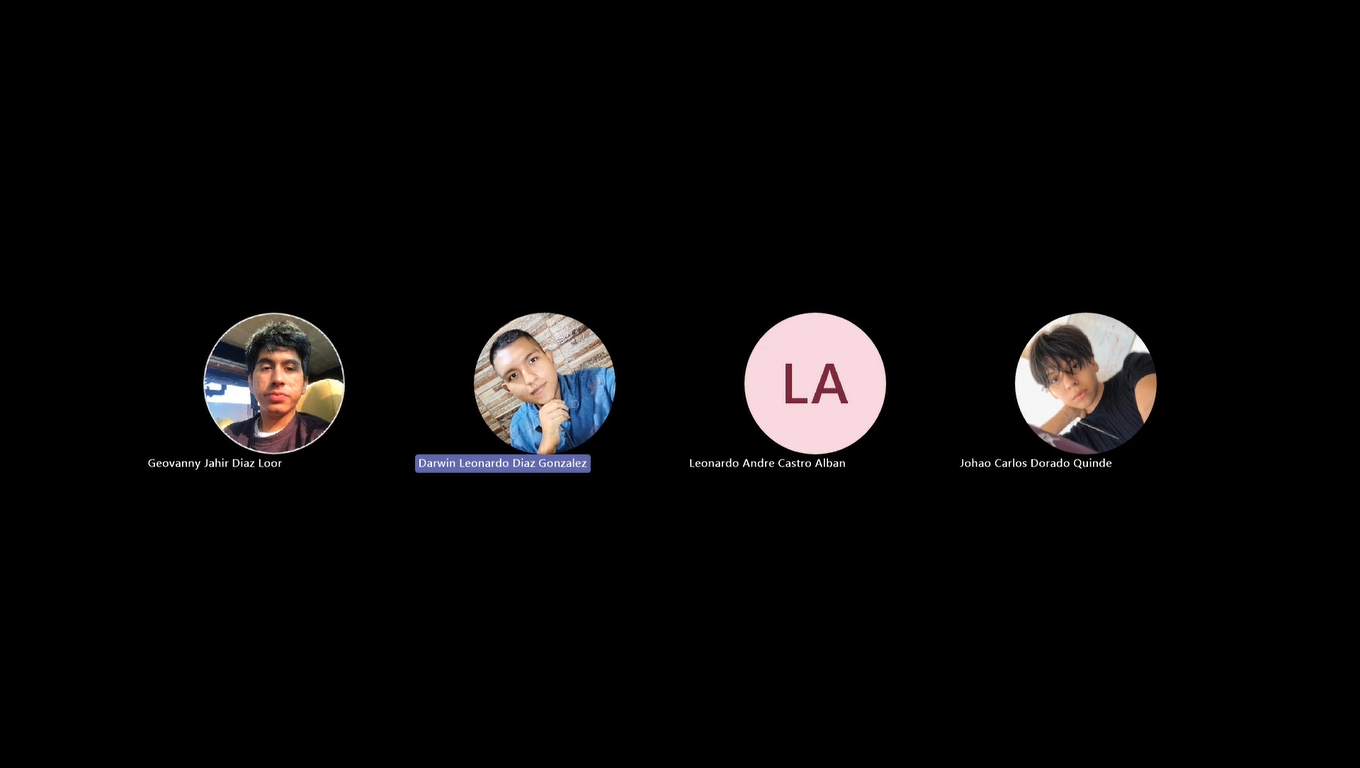
\includegraphics[width=0.85\linewidth]{imagenes/reunion_po_1.png}
\caption{Reunión 1 con el Product Owner -- 21 de mayo.}
\label{fig:reunion_po_1}
\end{figure}

\begin{figure}[H]
\centering
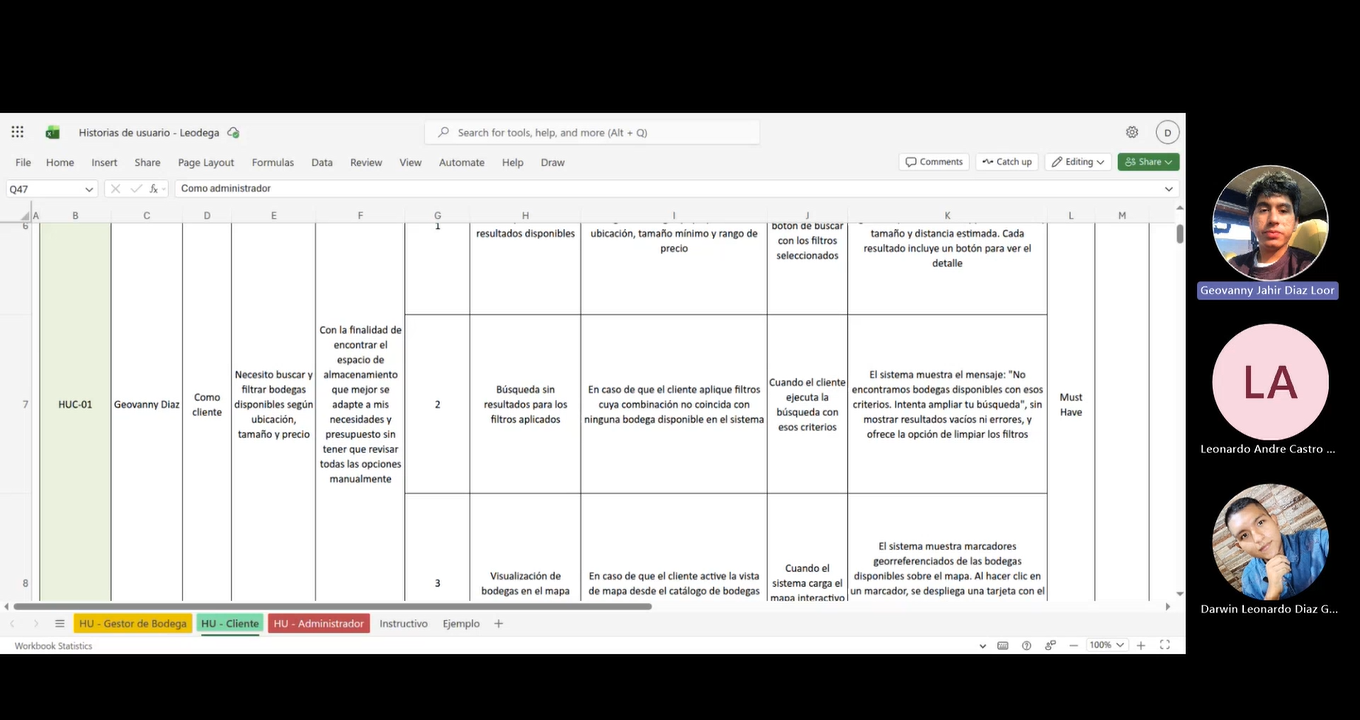
\includegraphics[width=0.85\linewidth]{imagenes/reunion_po_2.png}
\caption{Reunión 2 con el Product Owner -- 29 de mayo.}
\label{fig:reunion_po_2}
\end{figure}

\begin{figure}[H]
\centering
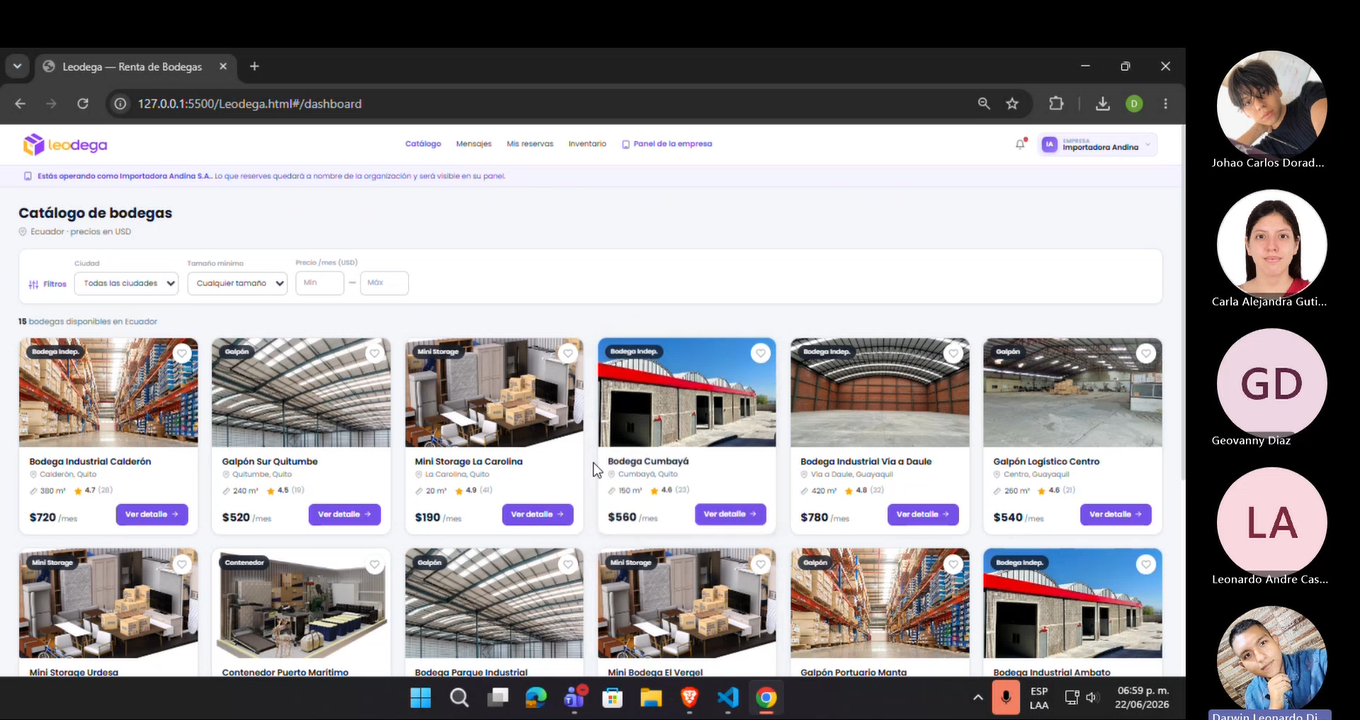
\includegraphics[width=0.85\linewidth]{imagenes/reunion_po_3.png}
\caption{Reunión 3 con el Product Owner -- 22 de junio.}
\label{fig:reunion_po_3}
\end{figure}
